% Apology to reader:

% The indentation in here is extremely weird, and you can see
% me struggle with trying to establish an indentation that I'm happy with. I
% once upon a time used to LaTeX with monstrous hundred or even thousand
% character lines, but I'm trying to move to a more code-like structure, and
% this document is a living testament to my struggles :(
    \documentclass[12pt]{report}
    \usepackage{fancyhdr, amsmath, amsthm, amssymb, mathtools, lastpage,
    hyperref, enumerate, graphicx, setspace, wasysym, upgreek, listings,
    fouriernc}
    \usepackage[margin=1in]{geometry}
    \usepackage{float}
    \newcommand{\scinot}[2]{#1\times10^{#2}}
    \newcommand{\bra}[1]{\left<#1\right|}
    \newcommand{\ket}[1]{\left|#1\right>}
    \newcommand{\dotp}[2]{\left<#1\,\middle|\,#2\right>}
    \newcommand{\rd}[2]{\frac{\mathrm{d}#1}{\mathrm{d}#2}}
    \newcommand{\pd}[2]{\frac{\partial#1}{\partial#2}}
    \newcommand{\rtd}[2]{\frac{\mathrm{d}^2#1}{\mathrm{d}#2^2}}
    \newcommand{\ptd}[2]{\frac{\partial^2 #1}{\partial#2^2}}
    \newcommand{\norm}[1]{\left|\left|#1\right|\right|}
    \newcommand{\abs}[1]{\left|#1\right|}
    \newcommand{\pvec}[1]{\vec{#1}^{\,\prime}}
    \newcommand{\tensor}[1]{\overleftrightarrow{#1}}
    \let\Re\undefined
    \let\Im\undefined
    \newcommand{\ang}[0]{\text{\AA}}
    \newcommand{\mum}[0]{\upmu \mathrm{m}}
    \newcommand{\bm}[1]{\boldsymbol{\mathbf{#1}}}
    \DeclareMathOperator{\Re}{Re}
    \DeclareMathOperator{\Res}{Res}
    \DeclareMathOperator{\Im}{Im}
    \DeclareMathOperator{\Log}{Log}
    \DeclareMathOperator{\Arg}{Arg}
    \DeclareMathOperator{\diag}{diag}
    \DeclareMathOperator{\Tr}{Tr}
    \DeclareMathOperator{\E}{E}
    \DeclareMathOperator{\Var}{Var}
    \DeclareMathOperator*{\argmin}{argmin}
    \DeclareMathOperator*{\argmax}{argmax}
    \DeclareMathOperator{\sgn}{sgn}

    \DeclarePairedDelimiter\p{\lparen}{\rparen}
    \DeclarePairedDelimiter\s{\lbrack}{\rbrack}
    \DeclarePairedDelimiter\z{\lbrace}{\rbrace}

    \newcommand{\expvalue}[1]{\left<#1\right>}
    \usepackage[labelfont=bf, font=scriptsize]{caption}\usepackage{tikz}
    \usepackage[font=scriptsize]{subcaption}
    \everymath{\displaystyle}

\tikzstyle{circ} = [draw, circle, fill=white, node distance=3cm, minimum
height=2em]

\definecolor{commentgreen}{rgb}{0,0.6,0}
\lstset{
    basicstyle=\ttfamily\footnotesize,
    frame=single,
    numbers=left,
    showstringspaces=false,
    keywordstyle=\color{blue},
    stringstyle=\color{purple},
    commentstyle=\color{commentgreen},
    morecomment=[l][\color{magenta}]{\#}
}

\begin{document}

\pagestyle{fancy}
\rhead{Yubo Su --- Tidbits}
\cfoot{\thepage/\pageref{LastPage}}

Welcome back to my random tidbits file! When I come up with interesting
problems, I will put them here.

\tableofcontents

\chapter{Probability Distributions and Weight Loss}

I was keeping track of my own weight when I realized that my scale was
sufficiently inconsistent that my weight loss was dominated by the statistical
noise. So then I was curious what the best way of mitigating this is, mean or
median of multiple measurements. One would suspect it's the mean, or one would
know simply by having taken any real statistics class, but I'm curious.

\section{Mean-based averaging}

This one is easy. Assume we have $n$ iid variables $X_i$ with mean $\mu$ and
variance $\sigma^2$, then the random variable corresponding to their average
$\expvalue{X_i}$ has mean $\mu$ and variance $\frac{\sigma^2}{n}$, so standard
deviation $\frac{\sigma}{\sqrt{n}}$. Thus, we have an unbiased estimator of the
true mean and a variance that falls off like $\sim n^{-1/2}$.


\section{Median-based averaging}

This one is a bit more fun. Let's start with $n=3$, then defining $f(x)$ the
probability density function and $F_X(x) = f_X(X \leq x)$ the cumulative
distribution function, the probability density of the median $f_\eta(y)$ is
given
\begin{align}
    f_\eta(y) = 6f_X(y)F_X(y)\left( 1 - F_X(y) \right)\label{1-eta}
\end{align}
the probability we choose one value greater than $y$ the median and one less,
multiplied by $6$ because there $3$ ways to choose which element is the median
and $\binom{2}{1}$ binomial coefficient for exactly one element on each side.
This seems to be a bit difficult to verify to be normalized in the general case,
or that
\begin{align}
    \int\limits_{-\infty}^{\infty}f_\eta(y)\;\mathrm{d}y &=
    \int\limits_{-\infty}^{\infty}\left[
        6f_X(y)\int\limits_{-\infty}^{y}f_X(\xi)\;\mathrm{d}\xi
        \int\limits_{y}^{\infty}f_X(\zeta)\;\mathrm{d}\zeta
    \right]\mathrm{d}y = 1
\end{align}

Let's just verify this in the uniform distribution case, and leave the general
oase as an exercise to brighter colleagues. We consider the normalized uniform
distribution $f_X(x) = 1, x \in [0,1]$, or $F_X(x) = x, x \in [0,1]$. We confirm
that the expression for $f_\eta$ is normalized:
\begin{align}
    \int\limits_{0}^{1}6y(1-y)\;\mathrm{d}y = 1
\end{align}

We then wish to examine whether $f_\eta(y)$ is an unbiased estimator of $\mu$.
Again, we begin with examining a sub-case, where $f_X(x)$ is symmetric about its
mean $\mu$. This yields that $F_X(\mu) = 0.5$ and is odd about
$\mu$\footnote{This is a slight abuse of terminology: we mean that $F_X(x - \mu)
- 0.5 = -(F_X(-(x-\mu)) - 0.5)$.} and so that $F_X(y)\left( 1 - F_X(y) \right)$
is also even/symmetric about $\mu$. Finally, this implies that $f_\eta(y)$ as
defined in \autoref{1-eta} is also symmetric about $\mu$ and we are done.

However, this analysis breaks down in the asymmetric case. We see that
$F_X(y)\left( 1 - F_X(y) \right)$ is \emph{always} symmetric about the
median $\eta$ of $f_X$, since $F_X(\eta) = 0.5$. In general, the mean and median
of a probability distribution are not equal, so there is no guarantee that
$\expvalue{f_\eta(y)} = \expvalue{f(y)}$, and indeed we can verify for some
contrived probability distribution such as
\begin{align}
    f_X(x) &=
    \begin{cases}
        2 & 0 \leq x \leq 0.25\\
        1 & 0.5 \leq x \leq 1\\
        0 & \text{else}
    \end{cases}
\end{align}
that $\expvalue{f_X(x)} = 0.4375$ while
\begin{align}
    \expvalue{f_\eta(y)} &= \int\limits_{0}^{0.25}24y^2(1-2y)\;\mathrm{d}y +
    \int\limits_{0.5}^{1}6y^2(1-y)\;\mathrm{d}y\\
    &\approx 0.4218
\end{align}

This should not have surprised us: we're trying to use a median to estimate the
mean of a distribution, and the two are equal when the PD is symmetric and
unequal otherwise.

The above analyses probably generalizes to median-of-$n$ trials, where with a
symmetric PD we have the being a unbiased estimator of the mean and with an
asymmetric an biased estimator, for any parity of $n$, but I'm too lazy to check
this out and will take it on faith. For reference, we assert the generalization
of \autoref{1-eta} below for odd $N = 2m+1$ trials below
\begin{align}
    f_{\eta, 2m+1}(y) &= N\binom{2m}{m} f_X(y)\left( F_X(y) \right)^m
        \left( 1 - F_X(y) \right)^m
\end{align}
which is simply generalizing to the concept of ``$m$ elements on either side of
$y$.''

It seems difficult to compare these median-based results (many of which could
probably be strengthened) to the mean based results in the case of an arbitrary
PDF, so let's specialize to a few tractable cases.

\section{Uniform Distribution}

I'm tired of not obtaining usable results, so let's simplify the discussion
considerably and assume that we have a uniform probability distribution, or that
$X \in [\mu - a, \mu + a]$. In this case the median-of-three also provides for
an unbiased estimator as shown above.  What is the variance of this estimator
then?

\subsection{Mean-based}

Let's first examine the results of a mean-based estimation of $\mu$. Call
$\hat{\mu}_N$ the estimator generated by averaging $N$ samplings, then we know
that $\expvalue{\hat{\mu}_N} = \mu$ by linearity of expectation and
$\sigma_{\hat{\mu}_N}^2 = \frac{\sigma_X^2}{N}$ by linearity of variance, so
it remains to compute $\sigma_X^2$, which is given by
\begin{align}
    \sigma_X^2 &= \expvalue{X^2} - \expvalue{X}^2\\
    &= \int\limits_{\mu - a}^{\mu + a}\frac{1}{2a}x^2\;\mathrm{d}x - \mu^2\\
    &= \frac{6\mu^2a + 2a^3}{6a} - \mu^2\\
    &= \frac{a^2}{3}
\end{align}

Thus, $\sigma_{\hat{\mu}_N}^2 = \frac{a^2}{3N}$.

\subsection{Median-based, $N=3$}

Now for the median-based approach. Denote $\tilde{\mu}_N$ the estimator
generated by taking the median of $N$ samplings, then we know that
$\expvalue{\tilde{\mu}_N} = \mu$ nonetheless because the uniform PD is a
symmetric probability distribution. It thus remains to compute
$\expvalue{\sigma^2_{\tilde{\mu}_N}}$. This seems nontrivial, so let's start
with $N=3$:
\begin{align}
    \expvalue{\tilde{\mu}_3^2} &= \int\limits_{-\infty}^{\infty}
        6f_X(x)F_X(x)\left( 1 - F_X(x) \right)\;x^2 \mathrm{d}x\\
        &= \int\limits_{\mu-a}^{\mu+a}
            \frac{6}{2a}\frac{x - (\mu - a)}{2a}\frac{(\mu + a) - x}{2a}x^2
            \;\mathrm{d}x\\
        &= \int\limits_{-a}^{a}\frac{6}{2a}\frac{a + y}{2a}\frac{a - y}{2a}
            (y + \mu)^2\;\mathrm{d}y\\
        &= \int\limits_{-a}^a\left[
                \frac{6}{8a^3}\left(
                    a^2y^2 + a^22y\mu + a^2\mu^2 - y^4 - 2\mu y^3 - y^2\mu^2
                \right)
            \right]\;\mathrm{d}y\\
        &= \frac{6}{8a^3}\left[
                \frac{(a^2 - \mu^2)y^3}{3} - \frac{y^5}{5}
            \right]_{-a}^a + \frac{3\mu^2}{2}\\
        &= \frac{6}{8a^3}\left[
            \frac{\left(
                a^2 - \mu^2
            \right) 2a^3}{3} - \frac{2a^5}{5}
        \right] + \frac{3\mu^2}{2}\\
        &= \mu^2 + \frac{a^2}{5}
\end{align}
and so $\sigma_{\tilde{\mu}_3}^2 = \frac{a^2}{5}$. Compare this to
$\sigma_{\hat{\mu}_3}^2 = \frac{a^2}{9}$ and we see that the mean-based
estimation has lower uncertainty.

\subsection{Median-based, arbitrary $N$}

Armed with this, let's also try to compute for arbitrary, odd $N=2m+1$, for which we
have
\begin{align}
    \expvalue{\tilde{\mu}_N^2}
        &=
            N\binom{2m}{m}\int\limits_{-a}^{a}\frac{1}{2a}
                \left( \frac{a^2 - y^2}{4a^2} \right)^m(y+\mu)^2
            \;\mathrm{d}y
\end{align}

Now, there's probably a cool combinatorial way to evaluate this, but let's just
care about asymptotic behavior. Then
\begin{align}
    \lim_{N \to \infty}\expvalue{\tilde{\mu}_N^2}
        &\approx
            N\frac{2^{2m}\sqrt{2m}}{m}\int\limits_{-a}^{a}
                \frac{1}{2a}\frac{1}{4^m}
                \left( 1 - \frac{y^2}{a^2} \right)^m (y+\mu)^2
            \;\mathrm{d}y\\
        &\approx \frac{1}{2a}\sqrt{8m}
            \int\limits_{-a}^{a}
                \left( 1 - \frac{y^2}{a^2} \right)^m(y+\mu)^2\;\mathrm{d}y
\end{align}
where we approximate $N \approx 2m$. Now, we know that $\left( 1-\frac{y^2}{a^2}
\right)^m$ is going to fall off sharply to $0$ as $y$ increases, so we can
approximate (for some normalization factor $A$)
\begin{align}
    \int\limits_{-a}^{a}\left( 1-\frac{y^2}{a^2} \right)^m\;\mathrm{d}y
        &\sim A
            \int\limits_{-a/\sqrt{m}}^{a/\sqrt{m}}
                1 - \frac{my^2}{a^2}
            \;\mathrm{d}y\label{1-two}\\
    \lim_{N \to \infty}\expvalue{\tilde{\mu}_N^2}
        &\approx \frac{A}{2a}\sqrt{8m}
            \int\limits_{-a/\sqrt{m}}^{a/\sqrt{m}}
                \left( 1 - \frac{my^2}{a^2} \right)(y+\mu)^2
            \;\mathrm{d}y
\end{align}
To compute $A$, we require that the coefficient of $\mu^2$ be $1$ so that the
difference $\expvalue{\tilde{\mu}_N^2} - \expvalue{\tilde{\mu}_N}^2$ does not
depend in first order on $\mu$. It's clear that since the integral is symmetric,
we need only consider even powers of $y$, and so our integral becomes
\begin{align}
    \lim_{N \to \infty}\expvalue{\tilde{\mu}_N^2}
        &= \frac{A\sqrt{8m}}{2a} \int\limits_{-a/\sqrt{m}}^{a/\sqrt{m}}
            \left( 1 - \frac{my^2}{a^2} \right)\left( y^2 + \mu^2 \right)
        \;\mathrm{d}y\\
        &= \frac{A\sqrt{8m}}{2a} \int\limits_{-a/\sqrt{m}}^{a/\sqrt{m}}
            \mu^2 + \left( 1 - \frac{m\mu^2}{a^2} \right)y^2 - \frac{my^4}{a^2}
        \;\mathrm{d}y\\
        &= \frac{A\sqrt{8m}}{2a} \left[
            \frac{2\mu^2a}{\sqrt{m}} + \left( 1 - \frac{m\mu^2}{a^2} \right)
                \left( \frac{2}{3}\frac{a^3}{m^{3/2}} \right) -
            \frac{2ma^5}{5a^3m^{5/2}}
        \right]\\
        &= A\frac{\sqrt{32}}{3}\mu^2 + A\frac{4\sqrt{2}}{15}\frac{a^2}{m}
\end{align}
and so we find that $A = \frac{3}{\sqrt{32}}$ and finally
\begin{align}
    \sigma_{\tilde{\mu}_N^2}^2 &= \frac{a^2}{5m}\label{1-result}
\end{align}

The agreement for $N=3, m=1$ is a bit uncanny, but let's try to verify this
computationally before jumping for joy.

This is a polynomial relationship on $m$, so we can sample $m$ logarithmically
to computationally verify our result. The obtained results are as follows in
\autoref{fig:1-medians}.
\begin{figure}[!h]
    \centering
    \begin{subfigure}{0.75\textwidth}
        \centering
        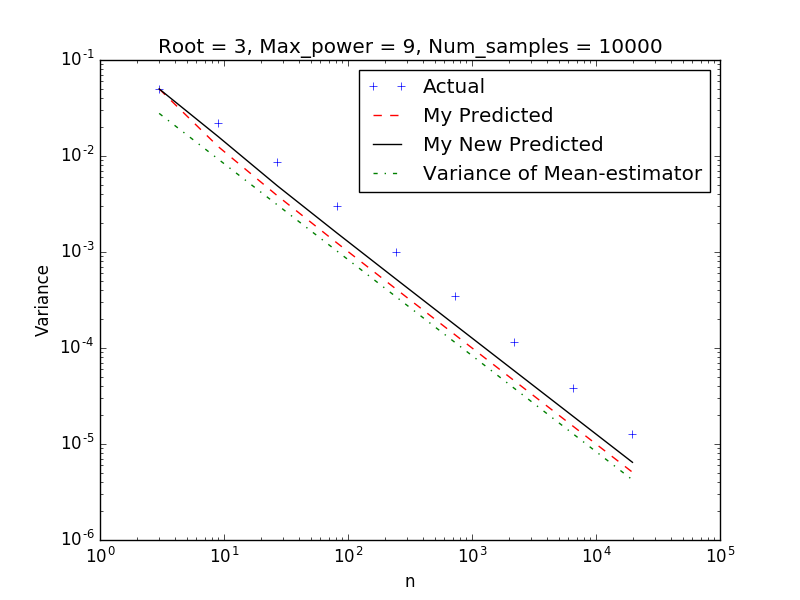
\includegraphics[width=\textwidth]{medians/medians_asymptotic.png}
        \caption{Plot of medians as a function of $N$}
    \end{subfigure}
    \begin{subfigure}{0.75\textwidth}
        \centering
        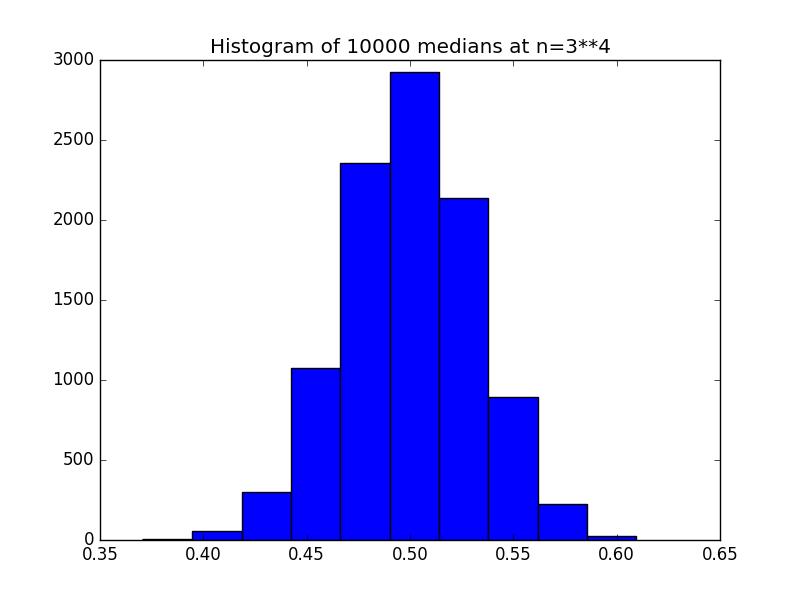
\includegraphics[width=\textwidth]{medians/medians_slice_hist.png}
        \caption{Histogram of $1000$ medians at a single value of $N$}
    \end{subfigure}
    \caption{Computational results for our medians result. Used $\mu=0.5,
    a=0.5$, or a uniform sampling $[0,1]$. Sampled over $n=3^{[1, 9]}$ with
    $10000$ samples at each value of $n$.}\label{fig:1-medians}
\end{figure}

The histogram is plotted merely out of curiosity, but seems to suggest a normal
distribution per the Law of Large Numbers. Nonetheless, \autoref{1-result}
seems to be slightly off. It perfectly agrees in the $N=3$ case as can be
verified by simulation, but eventually grows to be a factor of approximately $2$
off.

So it turns out our uncanny success for $N=3, m=1$ was a pure stroke of luck,
and our expression isn't precisely correct. Nonetheless, we can make a few plots
to figure out numerically how well median vs.\ mean based averaging performs,
and the degredation of our estimate over $N$. These plots are
\begin{figure}[!h]
    \centering
    \begin{subfigure}{0.45\textwidth}
        \centering
        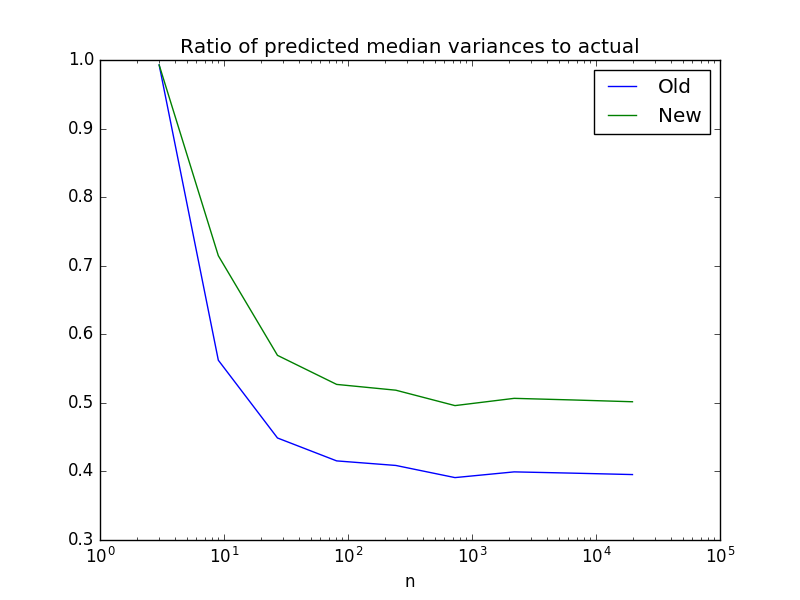
\includegraphics[width=\textwidth]{medians/medians_ratio_to_real.png}
        \caption{Seems asymptotically close to $2/5, 1/2$ maybe?}
    \end{subfigure}
    \begin{subfigure}{0.45\textwidth}
        \centering
        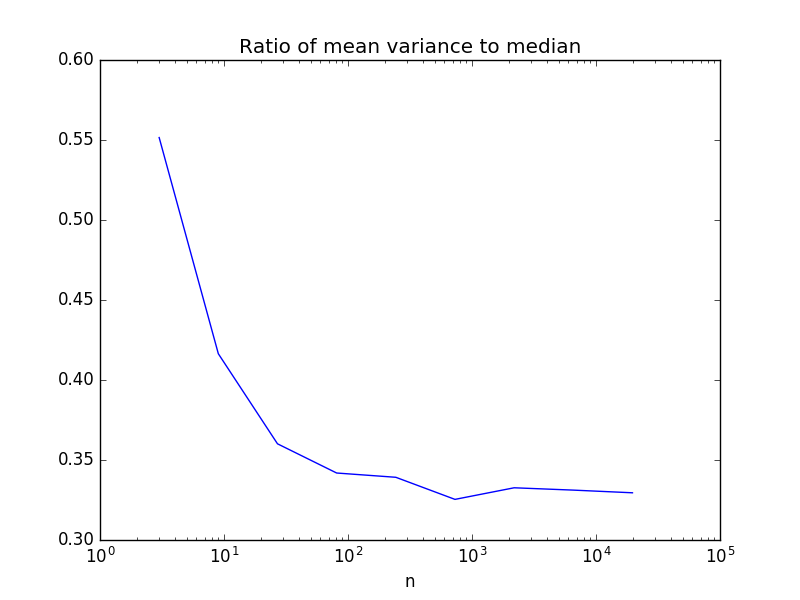
\includegraphics[width=\textwidth]{medians/medians_ratio_to_mean.png}
        \caption{Seems asymptotically close to $1/3$?}
    \end{subfigure}
    \caption{A couple ratios of interest. Same sampling as in
    \autoref{fig:1-medians}.}\label{fig:1-ratios}
\end{figure}

\subsection{Median-based, arbitrary $N$, reworked}

Let's try to include the truncated terms in $\left( 1 - \frac{y^2}{a^2}
\right)^m$, since they really are rather non-small compared to the leading term
that we kept. Where we had before put $1 - \frac{my^2}{a^2}$, we should instead
put
\begin{align}
    \left( 1 - \frac{y^2}{a^2} \right)^m
        &= \sum\limits_{k=0}^{m} \binom{m}{k}\left( -\frac{y^2}{a^2} \right)^k\\
    \lim_{N \to \infty}\expvalue{\tilde{\mu}_N^2}
        &\approx \frac{A}{2a}\sqrt{8m}
            \int\limits_{-a/\sqrt{m}}^{a/\sqrt{m}}
                \sum\limits_{k=0}^{m}\binom{m}{k}
                    \left( -\frac{y^2}{a^2} \right)^k
                (y+\mu)^2
            \;\mathrm{d}y
\end{align}

We approximate $\binom{m}{k} \approx \frac{m^k}{k!}$ since higher terms in $k$
are attenuated anyways. Using the same parity argument to kill the term odd in
$y$, we rewrite
\begin{align}
    \lim_{N \to \infty}\expvalue{\tilde{\mu}_N^2}
        &\approx \frac{A}{2a}\sqrt{8m}
            \int\limits_{-a/\sqrt{m}}^{a/\sqrt{m}}
                \sum\limits_{k=0}^{m}\frac{m^k}{k!}
                    \left( -\frac{y^2}{a^2} \right)^k
                (y^2+\mu^2)
            \;\mathrm{d}y
\end{align}

Examine first the $\mu^2$ coefficient
\begin{align}
    1
        &= \frac{A}{2a}\sqrt{8m}
            \sum\limits_{k=0}^{m}\frac{m^k}{k!}
                \int\limits_{-a/\sqrt{m}}^{a/\sqrt{m}}
                    \left( -\frac{y^2}{a^2} \right)^k
                \;\mathrm{d}y\\
        &= \frac{A}{2a}\sqrt{8m}
            \sum\limits_{k=0}^{m}\frac{m^k}{k!(2k+1)}
                2\left( \frac{a}{m^{k + 1/2}} \right)\left( -1 \right)^{k}\\
        &= A\sqrt{8}\sum\limits_{k=0}^{m}\frac{\left( -1 \right)^{k}}{k!(2k+1)}
\end{align}
and the other term
\begin{align}
    \lim_{N \to \infty}\sigma_{\tilde{\mu}_N}^2
        &\approx \frac{A}{2a}\sqrt{8m}
            \int\limits_{-a/\sqrt{m}}^{a/\sqrt{m}}
                \sum\limits_{k=0}^{m}\frac{m^k}{k!}
                    \left( -\frac{y^2}{a^2} \right)^k
                y^2
            \;\mathrm{d}y\\
        &= \frac{A}{2a}\sqrt{8m}
            \sum\limits_{k=0}^{m}\frac{m^k}{k!(2k+3)}
                2\left( \frac{a^3}{m^{k + 3/2}} \right)\left( -1 \right)^{k}\\
        &= \frac{A\sqrt{8}a^2}{m}\sum\limits_{k=0}^{m}
            \frac{\left( -1 \right)^{k}}{k!(2k+3)}\\
        &= \frac{a^2}{m}\frac{\
                \sum\limits_{k=0}^{m}\frac{\left( -1 \right)^k}{k!(2k+3)}
            }{\
                \sum\limits_{k=0}^{m}\frac{\left( -1 \right)^k}{k!(2k+1)}
            }\label{1-another_result}
\end{align}
and we find that we reproduce our previous result for $N=3$. Crunching the
numbers, we get something slightly better, though since factorials fall off so
quickly the change is very slight. The results are shown in
\autoref{fig:1-ratios}.

\subsection{Further ruminations (TBC)}

The approximation where we took the integral over interval $[-a/\sqrt{m},
a/\sqrt{m}]$ seems to be the last point of contention, as it bears noting that
if we allow a degree of freedom in the choice of range $\left[
    -Ba/\sqrt{m}, Ba/\sqrt{m}
\right]$ that our choice of $B$ propagates as a factor of $B^{2k+3}$ to the
summation in the numerator of \autoref{1-another_result} and $B^{2k+1}$ to the
summation in the denominator. Thus, our choice of $B$ has nontrivial
implications on the exact prefactor we obtain.

\section{Open Questions}

\begin{itemize}
    \item Is there any way to find the missing factor on median-based averaging
        for a uniform-distribution and arbitrary $N$?
    \item If we have discretized measurements, what are the statistics of
        mode-based averaging?
    \item Did I actually normalize the median-based averaging correctly, for a
        general probability distribution?
\end{itemize}

\section{Delta Function Properties}

I can never remember these, so I'll derive some of them below (used in PHYS7653
HW2, FA 2019). These are usually used for marginalizing over delta function
PDFs, so I'm not going to include any nontrivial integrand multiplying the
delta.
\begin{itemize}
    \item $\int \delta\p*{x - x_0}\;\mathrm{d}x = 1$ axiom.

    \item $\int \delta\p*{cx - y_0}\;\mathrm{d}x = \int \delta\p*{y -
        y_0}\;\mathrm{d}\frac{y}{c} = \frac{1}{c}$.

    \item $\int \delta\p*{f(x) - f_0}\;\mathrm{d}x = \int \delta\p*{f(x_0) - f_0
        + f'(x_0)(x - x_0)}\;\mathrm{d}x$ where $f(x_0) = f_0$, then applying
        above $= \frac{1}{f'(x_0)}$.

    \item $\int \delta\p*{f(x, y_i) - f_0}\;\mathrm{d}y_i$: this seems a little
        bit trickier, but I've actually included the generalization in
        \autoref{s:rand_var_dist}, it hinges on
        \begin{equation}
            \int \delta\p*{z - f(x_i)}\;\mathrm{d}^Nx_i =
                \int_{\mathcal{S}} \frac{1}{\hat{n} \cdot \vec{\nabla}
                    f(x_i)}\;\mathrm{d}^{N - 1}x_i.
        \end{equation}
        Note Wikipedia states the denominator as $\abs*{\vec{\nabla}f(x_i)}$,
        which is equivalent to our definition since $\hat{n}$ is the direction
        of steepest descent from $f(x_i)$; we will use their definition for
        clarity. We denote $\mathcal{S}$ to be the $N-1$ surface that satisfies
        constraint $f(x_i) = z$. This is always a little bit tricky to apply,
        since the units on the delta function matter, but using an integrand of
        $\delta\p*{\sqrt{\sum\limits_i x_i^2} - r}$ on the left hand side yields
        exactly $1$ for the integrand on the right hand side.

        Then the desired form is just
        \begin{equation}
            \int \delta\p*{f(x, y_i) - f_0}\;\mathrm{d}^Ny_i
                = \int\limits_{f(x, y_i) = f_0} \frac{1}{\abs{
                    \vec{\nabla} f\p*{x, y_i}}}\;\mathrm{d}^{N - 1}y_i.
        \end{equation}
        Note that the dot product in the denominator of the RHS must run over
        $x$ as well.

    \item $\int \delta\p*{f(x, y) - f_0} \delta\p*{g(x, y) -
        g_0}\;\mathrm{d}x\;\mathrm{d}y$: didn't end up using this one.
\end{itemize}

\chapter{Feynman-style number theory}

In case you have not yet seen
\url{http://www.lbatalha.com/blog/feynman-on-fermats-last-theorem} yet, it's
quite a fun read! Would recommend. That sort of thinking inspired this section.

\section{Asymptotic behavior of primes}

Call $\Pi(N)$ the prime number counting function, how many primes are below $N$.
The Prime Number Theorem is a well known result that postulates two
approximations to $\Pi(N)$:
\begin{align}
    \Pi(N) \approx \frac{N}{\log N} \approx \int\limits_{2}^{N}\frac{1}{\log
    x}\;\mathrm{d}x
\end{align}

We will attempt to derive the latter approximation. Consider $P(N)$ the
probability density that $N$ is a prime, roughly the statement ``if I randomly
choose a number near $N$, what is the probability it is a prime?'' The
relationship between $P(N)$ and $\Pi(N)$ is then
\begin{align}
    P(N) &= \rd{\Pi}{N}
\end{align}

To attempt to derive $P(N)$, consider that a number $N$ is prime iff it is not
divisible by any primes less than it. Thus, we have that
\begin{align}
    P(N) &\approx \prod_{p \in primes}^{N}\left( 1 - \frac{1}{p} \right)
\end{align}

Taking a leap of faith, we recognize that two consecutive contributions to the
product above differ roughly by $\frac{1}{P(p)}$, the local inverse probability
density that $p$ is prime. Thus, we can rewrite each contribution as
$\frac{1}{P(p)}$ contributions of $\left( 1 - \frac{1}{p} \right)^{P(p)}$, and
then allow $p$ to run over all integers. We thus propose the approximation
\begin{align}
    P(N) &\approx \prod_{k=2}^N\left( 1 - \frac{1}{k} \right)^{P(k)}
\end{align}

Taking the logarithm of both sides, we obtain
\begin{align}
    \log P(N) &= \sum\limits_{k=2}^{N}P(k)\log\left( 1 - \frac{1}{k} \right)
\end{align}

Approximating the right hand side with an integral, we obtain
\begin{align}
    \log P(N) &= \int\limits_{2}^{N}P(k)\log\left( 1 - \frac{1}{k}
    \right)\;\mathrm{d}k
\end{align}

Differentiating both sides now, we obtain
\begin{align}
    \frac{P'(N)}{P(N)} &= P(N)\log\left( 1 - \frac{1}{N} \right)\\
    \rd{P}{N} &= P^2\log\left( 1 - \frac{1}{N} \right)\\
    \frac{\mathrm{d}P}{P^2} &= \mathrm{d}N \log\left( 1 - \frac{1}{N} \right)\\
    -\frac{1}{P} &= N\log\left( 1 - \frac{1}{N} \right) - \log(N - 1)\\
    P(N) &= \frac{1}{\log(N - 1) + O(1)}\\
    &\approx \frac{1}{\log N}
\end{align}

This recovers the expression $\Pi(N) = \int\limits_{2}^{N}P(N)\;\mathrm{d}N =
\int\limits_{2}^{N}\frac{1}{\log N}\;\mathrm{d}N$.

\section{Scratch work}

\textbf{What follows is me working out loud, which is a lot less interesting.}

It's a well-known result (Prime Number Theorem) that the number of primes below
$N$ is approximated by $\Pi(N) = N/\log(N)$. Can we try to get a handle on this
behavior via application of continuum analysis?

One way of thinking of the problem is to instead look at it from a probabilistic
standpoint, that arbitrarily choosing a number $n$, it has some probability of
being prime. Can we estimate this probability and recover the prime number
theorem? We should be able to obtain
\begin{align}
    \rd{\Pi}{N} &\approx \frac{\log N - 1}{\log^2(N)}
\end{align}

\subsection{First attempt}

Let's consider the probability that some large number $N$ is divisible by some
divisor $d$; this is just $\frac{1}{d}$. We might think that the probability
that $N$ is prime then just the product of probabilities it is not divisible by
any number smaller than it
\begin{align}
    P(N) &= \prod_{k=2}^N \left( 1 - \frac{1}{k} \right)\label{2-prod}
\end{align}

To try to evaluate this product, we take the logarithm of both sides
\begin{align}
    \log P(N) &= \sum\limits_{k=2}^{N} \log \left( 1 - \frac{1}{k}
    \right)\\\label{2-intapprox}
    &\approx \int\limits_{k=2}^{N}\log \left( 1 - \frac{1}{k} \right)\;\mathrm{d}k\\
\end{align}

To compute this antiderivative, it's easiest to separate the integrand
\begin{align}
    \int\limits_{}^{}\log\left( \frac{k-1}{k} \right)\;\mathrm{d}k &=
    \int\limits_{}^{}\log (k-1)\;\mathrm{d}k - \int\limits_{}^{}\log
    k\;\mathrm{d}k\\
    &= (k-1)\log(k-1) - k - k\log(k) + k + C\\
    &= k\log\left( 1 - \frac{1}{k} \right) - \log(k-1) + C
\end{align}
with $C$ some undetermined constant that becomes irrelevant when we consider the
definite integral. Thus, we return to our primary expression
\begin{align}
    \log P(N) &\sim N\log\left( 1 - \frac{1}{N} \right) - \log(N - 1)
\end{align}
where we drop the evaluation of the antiderivative at $k=2$ since it's a
constant in the scaling. Then, we find
\begin{align}
    P(N) &\sim \frac{\left( 1 - \frac{1}{N} \right)^N}{N-1} =
    \frac{1/e}{N-1}
\end{align}

In fact, a quick google search shows that \autoref{2-prod} evaluates to
$\frac{1}{N}$, and so our result is pretty reasonable; we're off by a constant
factor since our integral approximation \autoref{2-intapprox} misestimates by a
constant factor, no surprise there. So where did we go wrong?

\subsection{Second attempt}

The iusse, as some people smarter than me may have noticed, is that our
expression \autoref{2-prod} is faulty: we should only be multiplying \emph{over
primes}! While this is correct, primes are not divisible by any primes smaller
than them, it's a bit difficult to handle under our present formalism, where we
only attach a probability to a number's being prime or not.

Let's think carefully about how to integrate this into our formalism. If a
number $k$ is not prime, it should contribute $1$ to our product, and if it is
prime then it should contribute $\left( 1 - \frac{1}{k} \right)$. Since we're
doing products, the natural way to ``average'' is via geometric mean, so we
modify expression \autoref{2-prod} to
\begin{align}
    P(N) &= \prod\limits_{k=2}^{N}\left( 1 - \frac{1}{k}
    \right)^{P(k)}\label{2-improved}
\end{align}
where we average each $k$-th contribution as $\left( 1 - \frac{1}{k}
\right)^{P(k)}(1)^{1-P(k)}$ geometric mean\footnote{Intuitively, this means that
we need to multiply $\frac{1}{P(k)}$ of these factors before getting a single
one that contributes, i.e.\ the distance between primes.}. Doing the usual trick,
\begin{align}
    \log P(N) &= \int\limits_{2}^{N}P(k) \log\left( 1 - \frac{1}{k}
    \right)\;\mathrm{d}k
\end{align}

Differentiating both sides,
\begin{align}
    \frac{P'(N)}{P(N)} &= P(N)\log\left( 1 - \frac{1}{N} \right)\\
    \rd{P}{N} &= P^2(N)\log\left( 1 - \frac{1}{N} \right)\\
    \frac{\mathrm{d}P}{P^2} &= \log\left( 1 - \frac{1}{N} \right)\mathrm{d}N\\
    -\frac{1}{P} &= N\log\left( 1 - \frac{1}{N} \right) - \log\left( N - 1
    \right)\\
    P(N) &\approx \frac{1}{\log N}
\end{align}

Interestingly, this expression is a better approximation to $\Pi(N)$ than the
aforementioned $\Pi(N) \approx \frac{N}{\log(N)}$, so it looks like this is a
satisfactory conclusion, namely that
\begin{align}
    \Pi(N) \approx \int\limits_{2}^{N}\frac{1}{\log(m)}\;\mathrm{d}m
\end{align}

However, we pursue one last direction of thought out of curiosity.

\subsection{Third attempt}

In \autoref{2-improved}, maybe we only need to check up until $\sqrt{N}$ in the
product. Continuing our thought above, we obtain
\begin{align}
    \frac{P'(N)}{P(N)} &= P(\sqrt{N})\log\left( 1 - \frac{1}{\sqrt{N}} \right)\\
    &\approx -\frac{P(\sqrt{N})}{\sqrt{N}}
\end{align}

At this point, our expression doesn't seem particularly amenable to solution,
but we can at least check how well $P(N) \sim \frac{1}{\log N}$ works:
\begin{align}
    \frac{-\frac{1}{N\log^2N}}{\frac{1}{\log N}} &= -\frac{2}{\sqrt{N}\log N}\\
    -\frac{1}{N\log N} &= \frac{2}{\sqrt{N}\log N}
\end{align}
which doesn't seem to work too well. How about the original estimate $P(N) \sim
\frac{\log N - 1}{\log^2 N}$?
\begin{align}
    \frac{\frac{2 - \log N}{N\log^3 N}}{\frac{\log N - 1}{\log^2 N}} &=
    - \frac{\frac{\log\sqrt{N} - 1}{\log^2\sqrt{N}}}{\sqrt{N}}\\
    \frac{2 - \log N}{N\log N \left( \log N - 1 \right)} &= \frac{2\left( 2 -
    \log N\right)}{\sqrt{N}\log^2 N}
\end{align}
which is even worse. The obvious problem is that the $\sqrt{N}$ has nowhere tho
go since the probability density $P$ depends only on the logarithm of $N$. So
interesting, considering the further optimization of only going up to $\sqrt{N}$
ruins the accuracy of our prediction!

\clearpage
\chapter{Ellipsoidal surface areas}

We all know that ellipses do not have a closed form for their arclength, but
their enclosed area is well defined, namely $A = \pi ab$. This can be seen by
defining an ellipse as a projection of a circle by unevenly scaling the axes,
and noting that an area element $\mathrm{d}x\mathrm{d}y$ scales linearly with
the projection factors.

One series approximation to the arclength can be computed by noting the
following: if $S$ is the arclength of an ellipse, then $S\mathrm{d}n$ for some
small $\mathrm{d}n$ estimates the change in area by enlarging the ellipse.

Systematically, exhibit an ellipse with axis lengths $a,b$, such that its area
is $\pi ab$. Then, say that we extend both axes by some $\mathrm{d}\epsilon$,
then its area becomes
$\pi ab + \pi (a+b)\mathrm{d} \epsilon + \mathcal{O}(\mathrm{d}\epsilon^2)$
, and the change in area is
$\pi (a+b) \mathrm{d}\epsilon + \mathcal{O}(\mathrm{d}\epsilon^2)$.
This implies that the arclength of an ellipse to first order is $\pi(a+b)$,
which seems to make sense for $a=b$.

This isn't particularly radical, and neither is this entire section, but we can
verify it to be reasonable for three dimensions as well:
\begin{align}
    V &= \frac{4}{3}\pi abc + \frac{4}{3}\pi(ac + bc + ab)\mathrm{d}\epsilon
        + \mathcal{O}(\mathrm{d}\epsilon^2)\\
    S &= \frac{4}{3}\pi\left( ac + bc + ab \right)
        + \mathcal{O}(\mathrm{d}\epsilon)
\end{align}
which again agrees with intuition for $a=b=c$

\clearpage
\chapter{12/04/16---Musings on Hamiltonian Chaos}

We learned in our chaos readings that given an integrable Hamiltonian (can be
written in terms of action-angle variables, has $N$ constants of motion for $2N$
dimensional phase space), a small perturbation generally breaks the toroidal
phase space trajectory into chaotic motion. Let's see how much of this we can
actually understand.

\section{Action-Angle variables}

I don't have my 106 notes handy, so let's rederive some action-angle stuff. The
archetypal Hamiltonian to use is the SHO $H = (p^2 + q^2)/2$. While we may have
suspicions for the choice of action-angle, we look up that
\begin{align}
    I &= \frac{1}{2\pi}\oint \mathrm{d}(pq)
\end{align}
the integral over one period. For us, let's note that
$E = H = \frac{p^2 + q^2}{2}$
is a constant of motion, thus we can write
\begin{align}
    p &= \sqrt{2E - q^2}\\
    I &= \frac{1}{2\pi} \left[ 2 \int\limits_{-\sqrt{2E}}^{\sqrt{2E}}
        \sqrt{2E - q^2}\;\mathrm{d}q \right]\\
    &= E
\end{align}
where we recognize the integral to just be the integral of the circle. This
makes sense, as we recognize that the action integral $I$ is just the area of
phase space enclosed within a full period, which for us is just $2\pi E$ since
we enclose a circle in phase space with radius $r^2 = 2E$.

The angle $\theta$ must be such that the above expression also holds, i.e.
\begin{align}
    \oint \mathrm{d}(pq) &= \oint \mathrm{d}(I\theta)
\end{align}
so that the phase space volume enclosed in one rotation is the same for both
variables. We can then differentiate both sides by $I$ to obtain
\begin{align}
    \theta &= \pd{}{I}\oint \mathrm{d}pq.
\end{align}

Since the $\oint$ depends only on the bounds of integration, we see that
$\theta$ is simply the limit on the integral, which further algebra shows to be
$\arctan \frac{q}{p}$. We can verify that this is canonical by computing the PB
\begin{align}
    \pd{I}{p}\pd{\theta}{q} - \pd{I}{q}\pd{\theta}{p} &=
        p \frac{1}{p}\frac{1}{1 + \left( \frac{q}{p} \right)^2} -
        q \left( - \frac{q}{p^2} \right)
        \frac{1}{1 + \left( \frac{q}{p} \right)^2}\\
    &= 1
\end{align}
so we're in good shape.

\section{Multi-dimensional SHOs}

In more generality, if we have a multidimensional SHO, we see that the
Hamiltonian is just their sum, and so $H$ in terms of action angle variables is
still the sum of the actions, while their angles evolve separately.

What is the rate at which the angle evolves? For our above single-dimensional
oscillator, it's easy to simply solve the EOM and find that $\frac{q}{p} = \tan
t$, and so that the angle evolves with unit frequency. More generally, if the
Hamiltonian is of form $H = p^2 + Cq^2$, it is easy to associate $C = \omega^2$
thanks to Hamilton's canonical equations $\dot{p} = H_q, \dot{q} = -H_p$ or
something like that up to a sign. Thus, in general our Hamiltonian takes on form
\begin{align}
    H &= \frac{\sum_j p_j^2 + \omega_j^2q_j^2}{2} = \sum_j \omega_j I_j
\end{align}
with each of the $I_j$ having a corresponding angle $\theta_j$ that evolves at
$\omega_j$.

\section{With perturbation (incorrect result and faulty method)}

How can we handle the perturbation? I have no idea, but I'll give it a shot.
Let's adopt a phase space where each $(q_j, p_j)$ are components of a complex
number. Then the $I_j$ are the magnitudes of each component, the $\theta_j$ the
phases, and the Hamiltonian acts simply to rotate each component. It's easy to
write down a system of equations that reproduces this behavior, but can we
express it in terms of the Hamiltonian? Put another way, is there a way we can
cast the $2N$-dimensional real Hamiltonian system above into an $N$-dimensional
complex system with similar rules?

The defining property of a Hamiltonian system is Hamilton's canonical equations
$\dot{p} = \pd{H}{q}, \dot{q} = -\pd{H}{p}$. If each dynamical variable is
instead $z_j = p_j + iq_j$, we instead want a property that looks something like
$\dot{z}_j = i\pd{H}{z_j}$\footnote{We have made a choice of convention in
putting the $i$ with the partial derivative rather than in the Hamiltonian,
motivated by keeping the Hamiltonian clean and most in analog with the
real-variable Hamiltonian}.

Specializing to the SHO, given an $\omega$ in the SHO, we should make the
correspondence $z_j = p_j + i\omega_jq_j$. Then we can write $H = \sum_j
\omega_j z_j^2/2$ which gives us results something like
$\dot{p}_j = -\omega_jq_j, \omega_j\dot{q}_j = p_j$ which is in accordance with
what we expect. Thus, for an SHO we have
\begin{align}
    \dot{z_j} &= i\pd{H}{z_j} = i\omega_jz_j
\end{align}

In other words, the evolution of the system is fully diagonal with eigenvalues
$\omega_j$. This is awfully reminescent of quantum mechanics! However, in QM,
first order perturbation theory always gives us a result for a new orthogonal
basis; why would any tori in classical mechanics break down? What does it even
mean for a torus to break down? Why am I so stupid? These are not rhetorical
questions but rather live musings as I type this up.

Consider if we then perturb the above EOM to something like
\begin{align}
    \dot{z}_j &= i\omega_jz_j + i\epsilon \pd{\delta
    H\left(\vec{z}\right)}{z_j}
\end{align}

Let's do the sensible thing and linearize $\delta H$ so that
$\delta H(\vec{z}) = \delta \mathbf{H}\vec{z}$. We seek a new set of $z_j$
such that the EOM is again diagonal. If we treat the $z_j$ coordinates as
vectors in a vector space, we can do this via perturbation theory
analogous to QM\@. Let's write down ansatz for new eigenbasis
\begin{align}
    \vec{z}_j &= \vec{z}_j + \sum_kA_{jk}\vec{z}_k
\end{align}

We then seek that $\pd{(\mathbf{H} + \delta \mathbf{H})(\pvec{z}_j)}{z'_j} =
\omega_j' \pvec{z}_j$, and so (goodness the algebra below is so so wrong, but
suck it up)
\begin{align}
    \pd{\mathbf{H}\vec{z}_j}{z_j} + \pd{\delta \mathbf{H}\vec{z}_j}{z_j} +
        \pd{}{z_j}\mathbf{H}\sum_k A_{jk}\vec{z}_k
        &= \omega_j z_j\hat{\jmath} + \delta
        \omega_j \vec{z}_j + \omega_j \sum_k A_{jk}\vec{z}_k\\
    \sum_k (\delta H)_{kj}\hat{k} + \sum_kA_{jk}\omega_k \vec{z}_k &=
        \delta \omega_j z_j\hat{\jmath} + \omega_j \sum_k A_{jk}\vec{z}_k\\
    A_{jk} &= \frac{(\delta H)_{jk}}{\omega_j - \omega_k}
\end{align}
which is in line with the result from QM\@. I don't trust the algebra but I
think the result is reasonable.

Not really sure where to go from here, but I found old lecture notes on the
topic so I'll just consult them. Oops. It's been fun!

The correct approach (which we may or may not work through) attacks this from
the generating function perspective, computing the Hamilton-Jacobi generating
function for the canonical transformation in terms of the small perturbation,
then showing that for purely rational $\omega_j$, the perturbation theory fails
to converge. It would appear then that the transformation of coordinates we
propose above in general is not canonical for a rational winding number or
something like that, if $H_1$ has a sufficiently high frequency component.

The moral of the story is that in classical mechanics, to change coordinates we
must approach from a generating function to show that the transformation is
canonical. Duly noted.

I continue this discussion in a separate section in my chaos notes, and conclude
this discussion to pursue more interesting musings about the classical-quantum
correspondence we began to uncover above.

\clearpage

\chapter{12/07/16---Musings on Quantum-Classical correspondence}

I'll repeat a small amount of the earlier discussion for my own benefit as I
write this up.

The definiting characteristic of the Hamiltonian formalism are Hamilton's
canonical equations
\begin{align}
    \pd{H}{p_i} &= \dot{q}_i & \pd{H}{q_i} &= -\dot{p}_i
\end{align}

Above, we tried to map $z_i = q_i + ip_i$. However, part of what we did
incorrectly in the above section was to assume that $\pd{H}{z_i}$ exists, i.e.
$H$ is analytic in the $z_i$. This is generally not true, obviously, so we need
to do some work here.

I still want to try and make some sort of $z_i$ transformation, so let's
consider the following: let's try to construct some $\mathcal{H} = H + iH'$ such
that $\mathcal{H}$ is an analytic function of the $z_i = q_i + ip_i$. Recall the
Cauchy-Riemann equations for differentiability of a function $f(z) = u(z) +
iv(z), z = x + iy$:
\begin{align}
    \pd{v}{y} &= \pd{u}{x}& i\pd{v}{x} &= -i\pd{u}{y}
\end{align}
and so for us
\begin{align}
    \pd{H'}{p_i} &= \pd{H}{x_i}& \pd{H'}{q_i} &= -\pd{H}{p_i}
\end{align}

We then wish to compute $\pd{\mathcal{H}}{z_i}$. Since $\mathcal{H}$ is
analytic, it doesn't matter along which direction in the complex plane we
approach $z_i$, so we choose to fix $p_i$, and we obtain
\begin{align}
    \pd{\mathcal{H}}{z_i}\Bigg|_{p_i} &=
        \pd{H(q_i, p_i)}{q_i} + i\pd{H'(q_i, p_i)}{q_i}\\
        &= \pd{H}{q_i} - i\rd{H}{p_i}
\end{align}

Hey, that's super nice, since now we can write $\dot{z_i} =
-i\pd{\mathcal{H}}{z_i}$, or in slightly more familiar form
\begin{align}
    i\pd{z_i}{t} &= \pd{\mathcal{H}}{z_i}
\end{align}

But wait! We can do even better. Since for any $N$-dimensional system, we have
$N$ conserved quantities, we can always make canonical transformation for
$H(p_i, q_i) \to H(I_i)$ the action-angle transformation. I won't bother
checking canonical-ness here, but the new Hamiltonian $H(I_i) = \omega_iI_i$.

Furthermore, from here we can always make a canonical transformation $H(I_i) \to
H(a_i, b_i)$ where $a_i = \sqrt{2I_i}\cos\theta, b_i = \sqrt{2I_i}\sin\theta$
with $\theta$ the angle variable.  Let's verify that this is canonical
\begin{align}
    \pd{a_i}{I_i}\pd{b_i}{\theta_i} - \pd{b_i}{I_i}\pd{a_i}{\theta_i} &=
        \left( \frac{\cos\theta}{\sqrt{2I_i}} \right)
        \left( \sqrt{2I_i}(-\cos\theta) \right) -
        \left( \frac{\sin\theta}{\sqrt{2I_i}} \right)
        \left( \sqrt{2I_i}\sin\theta \right)\\
        &= -1
\end{align}
which means the Hamiltonian becomes
\begin{align}
    H &= \sum\limits_{i}^{}\frac{\omega_i}{2}(a_i^2 + b_i^2)
\end{align}
which is basically an SHO in $a_i, b_i$. But what's nice about this formulation
in particular is that
\begin{align}
    \pd{\mathcal{H}}{z_i} &= \pd{H}{a_i} - i\pd{H}{b_i}\\
    &= \omega_i(a_i + ib_i) = \omega_iz_i
\end{align}
and ergo we obtain
\begin{align}
    i\pd{z_i}{t} &= \omega_iz_i
\end{align}
which is exactly the Sch\"odinger equation in the energy eigenbasis! In other
words, write the matrix $H_{QM} = \diag(\hbar \omega_i)$, then we have
\begin{align}
    i\hbar \pd{\vec{z}}{t} &= H_{QM}\vec{z}\label{5.SE}
\end{align}

I'm off by a sign, which is simply a convention of the definition of $z_i$, or
alternatively a definiton on $i$. But we can start to see the emergence of the
QM interpretation: there are certain dynamical orbits that are invariant under
evolution by the Hamiltonian, and these correspond to the energy levels in QM
that have energy $\hbar \omega$ associated with them.

It should be noted in hindsight that our jubilance is slightly overeager: we
have showed that the Hamiltonian in classical mechanics can be interpreted to
dictate each component of $\vec{z}$ in a way that corresponds to $\omega_i$ the
rate of change of the angle variable, but we have in no way derived any energy
levels or the sort. This should not surprise us, as the quantization of energy
levels is a purely quantum mechanical phenomenon, but the resemblance
in~\autoref{5.SE} is still slightly superficial.

\section{Significance of $\pd{\mathcal{H}}{z_i} \Rightarrow H_{QM}\vec{z}$}

Note that to arrive at~\eqref{5.SE}, we made what amounted to the correspondence
$\pd{\mathcal{H}}{z_i} \Rightarrow \left( H_{QM}\vec{z} \right)_i$ up to
$\hbar$. This result makes perfect sense when $H$ is a quadratic sum of the
$q_i, p_i$, but how the hell do the other operators enter the picture?

It would seem that the key identification we must make here is how the complex
$\vec{z}$ vector relates to dynamical measurements in classical mechanics, since
the correspondence between $\vec{z}$ and state vector $\ket{\psi}$ is clear. In
order to measure, say, the $q_j$ position of the system given $\vec{z}$, we need
simply to compute the change-of-basis operation from the $z_i = a_i + ib_i$ to
the $q_i, p_i$ basis, then project out the $j$th index.

Another way to extract $q_j$ that perhaps seems more promising is to construct
the generating function $S$ (which exists for all canonical transformations).
Let's choose the generating function $S(a,b)$ such that $q = S_a, p=S_b$. It
seems clear that we can use the same complexification trick above to obtain a
$\mathcal{S}$ such that
\begin{align}
    q + ip &= \pd{\mathcal{S}(a + ib)}{(a+ib)}
\end{align}

Let's call $w=q+ip$, then we find that the $q_j$ component can be computed by computing
\begin{align}
    q_j &= \Re\left(-i\hat{w}_j \cdot \pd{\mathcal{S}}{\vec{z}}\right)
\end{align}
where I use the shorthand
$\left[ \pd{\mathcal{S}}{\vec{z}} \right]_j = \pd{\mathcal{S}}{z_j}$. Compare
this to the QM result, which would be $\dotp{q_j}{\psi}$, where in order to
evaluate the dot product we must compute the components of $\psi$ in the
$\left\{ q_j \right\}$ basis. We now interpret $\pd{\mathcal{S}}{\vec{z}}$ to be
the $\vec{z}$ under the basis tranformation dictated by $\mathcal{S}$. The
quantum mechanical equivalent of this operator would be $\sum_k
\ket{q_k}\bra{q_k}$ the resolution of identity but also the change of basis
operator.

There seems to be at first glance a trend here: quantum mechanical operators
tend to correspond to classical functions that act on a variable by
\emph{differentiating} about that variable. In other words, the classical
correspondence of some operator $\Omega$ that acts on a wavefunction
$\ket{\psi}$ is $\mathbf{\Omega} = \pd{\Omega}{[~]}$ to be such that
$\mathbf{\Omega}\vec{v} = \pd{\Omega}{\vec{v}}$ and where $\Omega$ is some
complexified analytic function of its real/Hamiltonian counterpart. We have seen
this to be true for the resolution of identity and for the Hamiltonian itself.

Let's note that, heuristically, this explains the mapping of Poisson Brackets
to commutators. Recall that a set of coordinates is classically canonical if its
PB with $q,p$ is unity, and a set of variables is conjugate if their commutator
is $i\hbar$. These are both phase space-preserving constraints, so it's clear
that the latter is really the stipulation that the commutator of conjugate
variables must equal $\left[ X,P \right] = i\hbar$, just as the PB is just that
the change of coordinates has Jacobian with unit determinant. Let's try to flesh
this out a bit more.

\section{Classical Observables and Quantum Mechanical Operators}

Let's formalize the above a little bit. When we speak of a classical dynamical
variable $a$, it means that given a full specification of a state $\left\{ x_i,
p_i\right\}$, we can measure $a$ for the given state. Similarly, when we speak
of a quantum mechanical Hermitian operator (an observable) $A$, we mean that
given a $\ket{\psi}$ we can determine the probability of measuring $A$ given
$\ket{\psi}$ and observing any eigenvalue $\lambda$ of $A$, the probability
$\ket{\psi}$ is eigenstate $\ket{\lambda}$.

Under our above formalism, we mean the following: when we speak of a classical
dynamical variable $a$, we mean that the value of $a$ in a classical state
described by the complexified $\vec{z}_i$ can be computed by
\begin{align}
    a &= \Re\left(-i\hat{a}\cdot \pd{\mathcal{S}}{\vec{z}}\right)
\end{align}
where $\mathcal{S} = S + iS'$, $S$ being the generating function describing a
canonical transformation from $\left\{ x_i, p_i \right\}$ to some set of
canonical variables involving $a$ and $S'$ such that $\mathcal{S}$ is analytic.

For instance, if we want to compute $x_j$, we note that the generating function
has form $S = x_ip_i$, and so
\begin{align}
    \left[ \pd{\mathcal{S}}{\vec{z}} \right]_j &= \pd{\mathcal{S}}{z_j}\\
    &= p_j + ix_j\\
    x_j &= \Re(-i * (p_i + ix_j)) = x_j
\end{align}

The insertion of the $-i$ is a bit inconvenient, and clearly would have been
different were we trying to measure $p_j$. This seems a bit inconvenient, until
we remember that we can probably absorb these factors into $\mathcal{S}$ by
defining different operators; indeed, $X,P$ are different operators in QM, and
there seems to be little reason for us to use the same $\mathcal{S}$ for them!

Thus, under our formalism, classical dynamical variables $a$ map to second-order
tensors (matricies), which is again right for our correspondence.

As one last parting shot of the merit of our formalism, let's observe that if we
define a canonical transformation $\left\{ x_i, p_i \right\} \to \left\{ z_i,
z_i^* \right\}$ a classic trick, where $z_i = \frac{x_i + p_i}{\sqrt{2}}$, we
obtain that the PB is equal to $i$. The significance of this eludes me, but
certainly the agreement with QM up to an omnipresent $\hbar$ ought to be
encouraging?


\section{Normalizing the state vector}

An astute reader (all zero of you) would have objected a while ago that our
Hamiltonian only superficially resembled a quantum mechancical one, since as I
mentioned, the frequencies above correspond to the rate of change of the action
variable, which is a constant of the Hamiltonian and the \emph{system}, not the
state of the system. Contrast this with quantum mechanics, where the $\hbar
\omega$ eigenvalues of the Hamiltonian depend on the \emph{state} of the system
equally well as the Hamiltonian/configuration of the system itself.

We can see why we err: the $\omega$ above does not change when the amplitude of
motion changes, but the energy of the system clearly increases. To better
understand where this comes from, let's focus on a single dimension for now, so
two dimensions of phase space. If we recall how we wrote down the formula to
measure $x_j$ above, it relied on the fact that the $x_j$ component of some
vector was equal to the $x_j$ position of the taste. But $x_j \in \left(
-\infty,\infty \right)$, so this won't do if we try to normalize the state
vector. The only way we can get around this is by turning the single $x_j$
component into an infinity of components, one for each value of $x_j$. Then we
can ask whether the system's $x_j$ coordinate is some $x_0$ value by examining
whether the $x_0$ component is nonzero! (Now we see why we prefer to discuss
only a single dimension for now\dots)

Consider our system to be in a state $z_0 = x_0 + ip_0$, and map it to a
continuous function $\psi(z=x+ip) = \delta(x-x_0)\delta(p-p_0)$. It is easy to
verify that $\psi$ is normalized $\int \abs{\psi^2} = 1$, and we may measure the
position of $\psi$ by integrating it against an operator
\begin{align}
    x_0 &= \int x \abs{\psi}^2 \;\mathrm{d}x\mathrm{d}p
\end{align}

Lest I be accused of cherry-picking my normalization criterion for $\psi$, I
remind you this is the standard normalization procedure for vectors. My argument
above holds equally well whether using $\int \psi$ or $\int \abs{\psi}^2$, since
we're only dealing with $\delta$ functions. So I guess it's a tossup.

We can find similar expressions to measure the energy etc.\ of the system, and we
see that we have moved from a $\mathbb{C}^n$-component vector representation of
the state of the system to a representation that has unit norm albeit is a
continuous function on $\mathbb{C}^n$. One can easily contest that this is an
obfuscation of the physics, but is a natural starting ground for quantum
mechanical states, where the phase space is discretized and we can have linear
superpositions of states.

\section{Afterword}

We are officially at an impasse: without foresight of the quantization that
quantum mechanics brings, without supposing that systems have finite precision
in conjugate dynamical variables, it is impossible to proceed. These assumptions
have no place in a classical worldview, and it seems that we have largely
exhausted the range of speculations we can accomplish. But what a rich theory it
is already! We have shown that it is possible to
\begin{itemize}
    \item Map a $2N$ real phase space to a normalized state vector without
        losing any expressiveness.

    \item Proposed a second-order tensor form for all classical dynamical
        variables that act similarly to quantum observables.

    \item Accidentally come across the canonical commutation relation and an
        eerily remeniscent version of the Schr\"odinger Equation.
\end{itemize}

A symplectic manifold is a system endowed with an antisymmetric two-form, called
the symplectic form. I think that this association of the antisymmetric two-form
with a complexified function is generalizable and perhaps broadly applicable as
a useful way of thinking about these two-forms. Of course, $n$-forms are
probably just generalizations of the complex numbers, on second thought, but
alas that is far beyond the scope of my intellect.

With this I close my analysis. Thanks for listening!

\chapter{12/14/16---Matricies}

We saw earlier in quantum chaos that the way that the continuous energy spectrum
breaks down into discrete eigenvalues (which governs the power spectrum of the
trajectory) is described by random matrix theory, specifically the distribution
of gaps between eigenvalues of random matricies follows the same distribution.
Let's see how much ground we can make on these results.

\section{Prelim: Distributions of combinations of random
variables}\label{s:rand_var_dist}

Suppose we want the difference of two random variables $X, Y$. For simplicity,
let's say that they're normally distributed. Of course, if we're just talking
expectation and variance then this is a trivial problem; how about the shape of
the distribution? Differences of normal variables are also normally distributed,
but let's see one way we can describe this. Call $Z = X - Y$, with both $X,Y$
chosen with zero mean and standard deviation $\sigma$, then we should obtain
\begin{align}
    P_Z(z) &= \iint P_X(x) P_y(y) \delta(x - y - z)\;\mathrm{d}x\mathrm{d}y\\
    &= \int\limits_{-\infty}^{\infty}P_X(x)P_y(x-z)\;\mathrm{d}x
\end{align}
and if we specialize $P_X = P_Y = N(0, \sigma)$ then (dropping normalizations)
\begin{align}
    P_Z(z) &\propto \int\limits_{-\infty}^{\infty}e^{-\frac{x^2}{2\sigma^2}}
        e^{-\frac{(x-z)^2}{2\sigma^2}}\;\mathrm{d}x\\
    &\propto \int\limits_{-\infty}^{\infty}
        \exp\left[ \frac{-(2x^2 - 2xz + z^2)}{2\sigma^2} \right]\;\mathrm{d}x\\
    &\propto \int\limits_{-\infty}^{\infty}e^{-\frac{2(x - z/2)^2}{2\sigma^2}}
        e^{-\frac{z^2/2}{2\sigma^2}}\;\mathrm{d}x
\end{align}
and since the former exponent integrates to a constant and the latter a Gaussian
of width $\sigma \sqrt{2}$, we haeve our answer. It is worth noting the former
exponent integrates to a constant with an extra factor of $\sqrt{2}$ that
provides exactly the correct normalization for the latter.

In fact, this is trivially generalizable. If we want the distribution of a
random variable $Z = f\left(\left\{ X_i \right\}\right)$ with each $X_i$ obeying
its own probability distribution $P_i(x_i)$, the distribution is simply
\begin{align}
    P_Z(z) &= \int \delta\left(z - f\left( \left\{ x_i \right\} \right)\right)
        \prod_i P_i(x_i)\;\mathbf{d}^N\vec{x}\\
    &= \int \frac{1}{\hat{n} \cdot \nabla f(x_i)}\prod_i P_i(x_i)\;
        \mathrm{d}^{N-1}\vec{x}
\end{align}

Thus, for any old $Z = f(X_i)$ we theoretically know how to compute the
distribution $P_Z(z)$. What if the probabilities are not independent though, or
similarly what if $f(X_i)$ is not differentiable? One such tricky example is $Z
= \max_i X_i$. Note that this problem is very similar to our eventual problem of
finding the distribution of \emph{differences} in eigenvalues, though perhaps
even more non-differentiable.

One interesting way to tackle this is to solve for the $U(0,1)$ uniform
distribution on the unit interval case, then apply to an arbitrary PDF by
mapping the two CDFs. This only works for a small number of distribution
functions at an analytic level however.

Instead, let's attack from this perspective: let's consider $P_Z(z)$ subject to
the assumption that $X_1 > X_2$. This is the probability $P_Z(z | X_1 \geq
X_2)$, which is simply $P_X(x | X \geq X_2) = \frac{P_X(x)}{P(x_2 \geq x)}$. If
we then define $C_X(x_0) = P_X(x \geq x_0)$ the CDF, the form of the solution is
simply
\begin{align}
    P_X(x | X > X_2) &= \frac{P_X(x)}{C_X(x)}
\end{align}

More generally, if we have $N$ iid variables distributed as $P_X(x)$, and we
want to compute their successive differences, then to compute the $k$th
largest value $X_k$ where the $X$ are ordered, we have
\begin{align}
    P_k(x_k) &= \frac{P_X(x)}{C_X^{k-1}(x)\left( 1-C_X(x) \right)^{N-k+1}}
\end{align}

\section{Back to matricies}

We've now laid out how to compute the distribution of a difference of two random
variables as well as the how to leverage the CDF to compute the $k$th largest
in a set of random variables. This is more than sufficient to generate the
distribution of differences of random variables; we really only need to compute
the distribution of the differences between two eigenvalues! Oops, did a bit of
extra work, though it was pretty fun.

We now must turn to exactly what the distribution of eigenvalues looks like.

\textbf{UNFINISHED}.

\chapter{12/16/16---Infinite Grid of Resistors}

It is a well known problem, \url{https://xkcd.com/356/}. Let's first attack this
problem under the continuous limit, to get some intuition for how to solve the
problem, then attack the discrete problem.

\section{Continuous Problem}

The problem is as follows: given an infinite plane with resistance $R = \rho L$,
what is the resistance between two points separated by distance $d$?

It would appear that the majority of the tools we have at our disposal to attack
such a problem allow us to compute $V$ the voltage everywhere given the voltage
at the two points separated by $d$. The current that the system draws is
directly related to the divergence of $V$ at the points of contact. The ratio
between these gives the effective resistance. Ok.

We know there are only two current sources, which means we know $\vec{\nabla}
\cdot \vec{J} = \sigma \vec{\nabla} \cdot \vec{E} = \sigma \vec{\nabla} \cdot
(\nabla V) = \sigma \nabla^2 V$ is just two delta functions, at the source and
sink. Moreover, we can look up the Green's function for a 2D infinite plane for
the Poisson Equation $\nabla^2 V = \delta(\vec{r} - \vec{r}_0)$. This alone
means we are given sufficient information to solve for $V(\vec{r})$ and with it
the effective resistance. Great!

I'll not do this exercise here since computing the GF is hard (ok, non-easy, not
really that bad) and using it is uninteresting yet grungy.

\section{Discrete Problem}

This is a much harder problem since we don't have the GF\@! Nor for that matter,
do we even have an equation of state like the Poisson Equation. Time to
translate that formalism.

Label each point $(i,j)$ discrete indicies, and call $V_{ij}$ the voltage at
$i,j$. We know that the voltage drop between two points is simply proportional
to the current, and we know that there are exactly one source and one sink in
the entire grid, so we have something like
\begin{align}
    V_{i+1,j} - 2V_{i,j} + V_{i-1,j} + V_{i,j+1} - 2V_{i,j} + V_{i,j-1} =
        R\left( \mathcal{J}_{ij} \right)
\end{align}
where $\mathcal{J}_{ij}$ we define to be the ``current source'' at $(i,j)$
(i.e.\ zero everywhere except $\pm$ unity at source/sink). This is just a
discrete version of the Poisson Equation.

Now we need the equivalent of the Green's Function. ACM95 style. We need to
develop the homogeneous equations first, then solve for the BVP at the boundary
induced by the delta function. We separate variables
\begin{align}
    V_{i+1,j} - 2V_{i,j} + V_{i-1,j} &= C_{ij}
\end{align}
where the only stipulation with $C_{ij}$ is that its negative goes into the $j$
coordinate of the separation of variables.

But wait, this is just the coupled SHO equation! So we will have an SHO along
one direction. Thus, $C_{ij}$ is simply $\lambda V_{ij}$ where $\lambda$ is
selected by the normal mode frequencies. What frequencies are allowed? Any
wavelength longer than $2a$ with $a$ the separation between nodes is allowed,
above the Nyquist frequency.

Seems like can solve now. \textbf{UNFINISHED}.

\chapter{04/28/17---Bridges,  Chains and others}

\section{Bridges and Dem Chainz}

Inspired by a visit to the Golden Gate bridge. I will first rehash a problem we
solved in a previous tidbits doc, then work on a new one.

\subsection{Shape}

Easy problem. What is the shape of a light chain holding up a horizontal bridge,
e.g.\ a suspension bridge? How about the shape of a chain freely suspended?

Consider first the former problem first, a light chain holding up a horizontal
bridge, as depicted magnificently in \autoref{fig:light_bridge}.
\begin{figure}[!h]
    \centering
    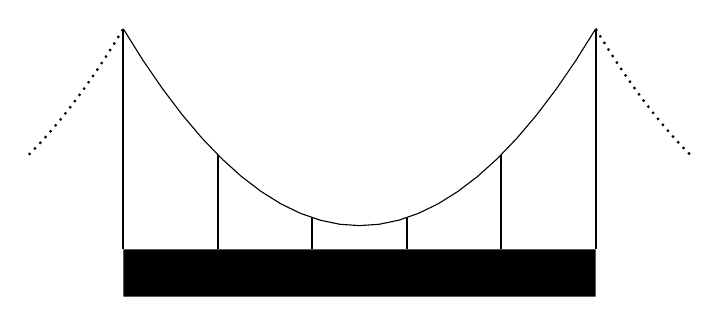
\begin{tikzpicture}[scale=0.3]
        \fill[black] (-10,1) -- (10,1) -- (10,-1) -- (-10,-1) -- (-10,1);
        \draw[domain=-10:10] plot(\x, {\x*\x/12 + 2});
        \draw[dotted, thick, domain=-14:-10] plot(\x, {(\x + 20)*(\x + 20)/12 + 2});
        \draw[dotted, thick, domain=10:14] plot(\x, {(\x - 20)*(\x - 20)/12 + 2});
        \draw[thick] (-10, 100 / 12 + 2) -- (-10, 1);
        \draw[thick] (-6, 36 / 12 + 2) -- (-6, 1);
        \draw[thick] (-2, 4 / 12 + 2) -- (-2, 1);
        \draw[thick] (2, 4 / 12 + 2) -- (2, 1);
        \draw[thick] (6, 36 / 12 + 2) -- (6, 1);
        \draw[thick] (10, 100 / 12 + 2) -- (10, 1);
    \end{tikzpicture}
    \caption{Picture of light chain holding up bridge.\label{fig:light_bridge}}
\end{figure}

Call the linear density of the bridge $\rho$. Let's compute $\vec{T}(x)$
the tension in the rope as a function of $x$, where $x \in [-L/2,L/2]$, $L$ the
distance between the supports. Because the setup is vertically symmetric, it
must satisfy $T_x(x) = -T_x(-x)$ i.e.\ it is odd, and $T_y(x) = T_y(-x)$ is
even.

At any point $x$, we know that $T_y(x + \mathrm{d}x) - T_y(x) = \rho \sgn(x)
(\mathrm{d}x)g$ the difference in $y$ components must support the differential
weight (where $\sgn(x)$ is the sign of $x$), or
\begin{align*}
    \rd{T_y}{x} &= \sgn(x)\rho g\\
    T_y(x) &= \rho g \abs{x}
\end{align*}

But then consider that $\vec{T}$ must lie along the chain, so $\frac{T_y}{T_x} =
\rd{y}{x}$. We note that $T_x$ must be constant almost everywhere, else the
chain would accelerate, but we note that it must point left on the left side and
right on the right side! We note that $T_x \propto \sgn(x)$ is thus what we are
looking for, and we obtain simply
\begin{align}
    \rd{y}{x} &= \frac{\rho g x}{\abs{T_x}} \nonumber\\
    y(x) &= \frac{\rho g}{2\abs{T_x}}x^2\label{eq:bridge_curve}
\end{align}
where we've chosen the constant of integration such that $y(0) = 0$. What
exactly is $T_x$ then? We see that it's the shape parameter; the looser the
chain is horizontally, the lower it drops, so given one we can compute the
other, but indeed a family of solutions exists for any $\rho, L$ determined by
their shape and tension.

\hrulefill

How about for a freely hanging chain, as in \autoref{fig:free_chain}?
\begin{figure}[!h]
    \centering
    \begin{tikzpicture}[scale=0.3]
        \draw[domain=-10:10] plot(\x, {\x*\x/12 + 2});
        \draw[dotted, thick, domain=-14:-10] plot(\x, {(\x + 20)*(\x + 20)/12 + 2});
        \draw[dotted, thick, domain=10:14] plot(\x, {(\x - 20)*(\x - 20)/12 + 2});
        \draw[ultra thick] (-10, 100 / 12 + 2) -- (-10, 1);
        \draw[ultra thick] (10, 100 / 12 + 2) -- (10, 1);
    \end{tikzpicture}
    \caption{Picture of free hanging chain.\label{fig:free_chain}}
\end{figure}

We have mostly the same math as before, except
\begin{align*}
    \rd{T_y}{x} &= \sgn(x) \rho g \sqrt{1 + \left( \rd{y}{x} \right)^2} &
    \frac{T_y}{T_x} &= \rd{y}{x}
\end{align*}
where the extra term comes in since $\mathrm{d}m = \rho (\mathrm{d}s) = \rho
\sqrt{\mathrm{d}x^2 + \mathrm{d}y^2}$ with $\mathrm{d}s$ the length of chain
which is also the \emph{arclength} now. We observe that
\begin{align*}
    \rd{T_y}{x} &= \rd{}{x}\left( T_x\rd{y}{x} \right) \\
    &= \abs{T_x}\sgn(x) \rtd{y}{x}
\end{align*}
and combining this with the above we obtain
\begin{align}
    \sgn(x) \rho g \sqrt{1 + \left( \rd{y}{x} \right)^2}
        &= \abs{T_x}\sgn(x)\rtd{y}{x}\nonumber\\
    \rtd{y}{x} &= \frac{\rho g}{\abs{T_x}}
        \sqrt{1 + \left( \rd{y}{x} \right)^2}\nonumber\\
    y(x) &= \frac{\abs{T_x}}{\rho g} \cosh
        \left( \frac{\rho g x}{\abs{T_x}} \right) + y_0\nonumber\\
    y(x) &= \frac{\abs{T_x}}{\rho g} \left(
        \cosh\left( \frac{\rho g x}{\abs{T_x}} \right)
        - 1\right) \label{eq:chain_curve}
\end{align}
and we see again $\abs{T_x}$ plays the role of a shape parameter and we've
chosen the solution such that $y(0) = 0$.

\textbf{Note:} We were a bit haphazard in asserting that $T_x(x) =
\abs{T_x}\sgn(x)$. It of course made sense, since at each point the $x$ tension
should be equal on both sides, meaning $\rd{T_x(x)}{x} = 0$, but we also knew
that $T_x(x)$ is odd. This is furthermore justifiable since it satisfies
$\vec{T}(0) = 0$, intuitive since the tension pulls in $\pm \hat{x}$ on either
side of $x=0$ which cancel, so any tension ``at'' $x = 0$ would produce an
acceleration. So it seems a justifiable conclusion.

\subsection{Force to Pull}

Let's hang these bridges and chains between two towers separated by a distance
$L$ such that the distance from the bottom of the chain to the top of the towers
is $h$. What is the tension in the chain? From this, we can compute what the
minimum force is to change $h$.

This is a simple exercise. $h$ is directly related to $T_x$, and from the shape
of the parabola we can get the ratio of $\frac{T_y}{T_x}$ and from this get
$\abs{\vec{T}}(h)$. So in the parabolic solution
\begin{align}
    h &= y\left( \pm \frac{L}{2} \right) = \frac{\rho g L^2}{8\abs{T_x}}
        \nonumber\\
    \abs{T_x} &= \frac{\rho g L^2}{8h}\nonumber\\
    \frac{T_y}{T_x} &= \rd{y}{x}\Bigg|_{x=L/2} = \frac{\rho g L}{2\abs{T_x}} =
        \frac{4h}{L}\nonumber\\
    \abs{\vec{T}} &= \sqrt{T_x^2 + T_y^2}\nonumber\\
    &= \abs{T_x}\sqrt{1 + \left(\rd{y}{x}\right)^2}\nonumber\\
    &= \frac{\rho g L^2}{8h}\sqrt{1 + \frac{16h^2}{L^2}}
\end{align}
and in the hyperbolic
\begin{align}
    h &= y\left( \pm \frac{L}{2} \right) = \frac{\abs{T_x}}{\rho g} \left(
        \cosh\left( \frac{\rho g L}{2\abs{T_x}} \right)
        - 1\right)
        \nonumber\\
    \frac{T_y}{T_x} &= \rd{y}{x}\Bigg|_{x=L/2} = \sinh \left(
        \frac{\rho g L}{2 \abs{T_x}}
    \right)\nonumber\\
    \abs{\vec{T}} &= \sqrt{T_x^2 + T_y^2}\nonumber\\
    &= \abs{T_x} \cosh \left( \frac{\rho g L}{2 \abs{T_x}} \right) \nonumber\\
    &= \rho g h + \abs{T_x}
\end{align}
and since we can't analytically solve for a relation between $\abs{T_x}, h$
we are probably stuck here. We can both in a couple limits though:
\begin{itemize}
    \item High $h$---For large $h$ in the parabolic case, the square root is
        roughly $\frac{4h}{L}$ and we obtain the trivial $\abs{\vec{T}} =
        \frac{\rho g L}{2}$ which is totally as expected: $\abs{T_x}$ vanishes
        as we grow higher, so we just need to support the weight of the bridge.

        For the hyperbolic case, large $h$ equates equates to large argument to
        the $\cosh$ which is for small $\abs{T_x}$ as in the parabolic case.
        This is again a dead end to evaluate analytically: the $\cosh$ goes to
        an exponential but then we're stuck. Instead, we see that $\abs{\vec{T}}
        \approx \rho g h$, which for large $h$ is roughly half the weight of the
        chain (since $h \gg L$, the length of the chain is approximately $2h$).

    \item Small $h$---For small $h$ in the parabolic solution, we have $T
        \propto h^{-1}$ so as we further shrink $h$, $T$ grows with its inverse.

        To get small $h$ for the hyperbolic case, we expect we need large
        $\abs{T_x}$, and indeed that lets us approximate
        \begin{align*}
            h
                &= \frac{\abs{T_x}}{\rho g}
                    \left(
                        \cosh\left( \frac{\rho g L}{2\abs{T_x}} \right) - 1
                    \right)\\
                &\approx \frac{\abs{T_x}}{\rho g}
                    \frac{\rho^2 g^2 L^2}{8 \abs{T_x}^2}
                    = \frac{\rho g L^2}{8\abs{T_x}}
        \end{align*}
        and we see that we recover the same limit as the parabolic solution,
        since at that point the chain's length is roughly $L$ as well and we
        have the same mass being suspended in both configurations.
\end{itemize}

To summarize, in the low $h$ case, both exhibit $\abs{\vec{T}} \propto h^{-1}$
behavior, but in the high $h$ case, the suspension bridge yields constant
tension while the chain yields $\abs{\vec{T}} \propto h$.

\section{Misc}

\subsection{Sum of Digits vs Base}

For large numbers, determine the dependence of the sum of the digits of the
number in some base $b$ as a function of $b$. When does the approximation break
down?

Let's just throw the simplest approximation we can at the problem first. For a
sufficiently large number, the distribution of one of its non-leading digits is
approximately uniform. Thus, in base $b$, the average digit is
$\frac{0 + 1 + \cdots + (b-1)}{b} = \frac{b - 1}{2}$. For any number $N$, the
number of digits is $\log_b N$, so we conclude that the sum of digits of $N$ in
base $b$ is approximately $S_b(N) = \frac{b - 1}{2}\log_b N$.

This seems to make sense: to build $S_b(N)$, we start with $S_b(0) = 0$, then we
can build $S_b(N)$ as
\begin{align*}
    S_b(b^i \leq N < b^{i+1}) = 1 + S_b(0 \leq N < b^i)
\end{align*}

Thus, $S_b(N)$ lies in the range  $\left[1, (b - 1)k\right]$ when $N$ is in the
range $[b^k, b^{k + 1} - 1]$ where $k$ is the number of digits in $N$ expressed
in base $b$, otherwise written $\lfloor \log_b N\rfloor$. What is the
distribtion of $S_b(N)$ in this range? That's simply the number of ways we can
pick $k$ numbers from $[0, b - 1]$ and sum them to $S_b(N)$.

We know that a single uniform distribution over $[0, b - 1]$ has mean $\frac{b -
1}{2}$ and variance $\frac{b^2 - 1}{12}$\footnote
{\url{https://en.wikipedia.org/wiki/Discrete_uniform_distribution}}, so
the sum of $k$ such variables has variance $\frac{k(b^2 - 1)}{12}$ since
variance is a linear operator. Thus, we obtain that the sum of digits of a
number $N$ in base $b$ has distribution
\begin{align}
    S_b(N)
        &= \frac{b - 1}{2}\log_b N \pm \sqrt{\frac{\log_b N (b^2 - 1)}{12}}\\
        &\approx
            \frac{b - 1}{2}\log_b N \left(1 \pm \sqrt{\frac{1}{3\log_b N}}
            \right)
\end{align}

Intuitively, this approximation fails when $\log_b N \sim b$, i.e.\ the number
of digits is of the same order as the number of possible digits, at which point
we can't assume each digit is uniformly distributed over $[0, b - 1]$ and
instead have to account for a greater concentration towards lower digits e.g.\
Benford's law.

% TODO distribution of sum of uniformly distributed random variables, continuous
% and discrete

\subsection{Approximations to Birthday Problem}

See what we can get for a back-of-the-envelope usable solution to the birthday
problem (draw with replacement from a set of size $N$, how many do you draw
before you expect a duplicate?).

If we draw $k$ elements with replacement from a set of size $N$, the probability
that we do not get any duplicates is $\frac{N!}{N^k(N - k)!}$. Throwing
Stirling's approximation at the two factorials, we obtain
\begin{align}
    P
        &\approx \sqrt{\frac{N}{N-k}}\left( \frac{N}{e} \right)^N
            \left( \frac{e}{N - k} \right)^{N - k} \frac{1}{N^k} \nonumber\\
        &= \left( \frac{N}{N - k} \right)^{N - k + 1/2}\frac{1}{e^k}
            \nonumber\\
        &= \left( 1 + \frac{k}{N - k} \right)^{N - k + 1/2}\frac{1}{e^k}
            \nonumber
\end{align}

We recall that $\left( 1 + \frac{k}{n} \right)^n$ as $n \to \infty$ is $e^k$,
but that would imply that $P > 1$. Instead, we have to recall that we canot take
the $N \to \infty$ limit since we're leaving out terms that themselves depend on
$N$.

Instead, let's find the first order correction to the log formula:
\begin{align}
    \log \left( 1 + \frac{k}{n} \right)^{n}
        \nonumber
        &= n\log \left( 1 + \frac{k}{n} \right)\\
        \nonumber
        &\approx n \left( \frac{k}{n} - \frac{k^2}{2n^2} + \mathcal{O}
            \left( \left(\frac{k}{n}\right)^3 \right)
        \right)\\
        \nonumber
        &= k - \frac{k^2}{2n}\\
    \left( 1 + \frac{k}{n} \right)^n &\approx \exp \left[
        k - \frac{k^2}{2n}\label{eq:e_approx}
    \right]
\end{align}
and so
\begin{align}
    P
        &= e^{-\frac{k^2}{2(N - k)}}\sqrt{1 + \frac{k}{N - k}}
\end{align}

How well does this do? We can compare the shape this curve produces with the
original $P = \frac{N!}{N^k(N-k)!}$, and we obtain
\begin{figure}[!h]
    \centering
    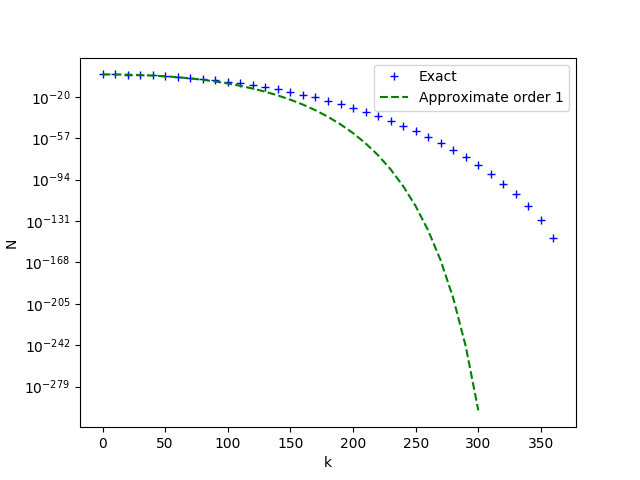
\includegraphics[width=0.7\textwidth]{birthdays/birthdays_approx.png}
    \caption{Plot of Exact and Approximate solutions for 365-day Birthday
        Problem\label{fig:birthdays}}
\end{figure}

So we see that at least in the regime $k \ll N$, we do reasonably well. We
recall that in~\eqref{eq:e_approx}, we only grabbed the first order term in
$\frac{k}{N}$; we can grab a few higher order terms and see what happens in
\autoref{fig:birthdays_higher_order}.
\begin{figure}[!h]
    \centering
    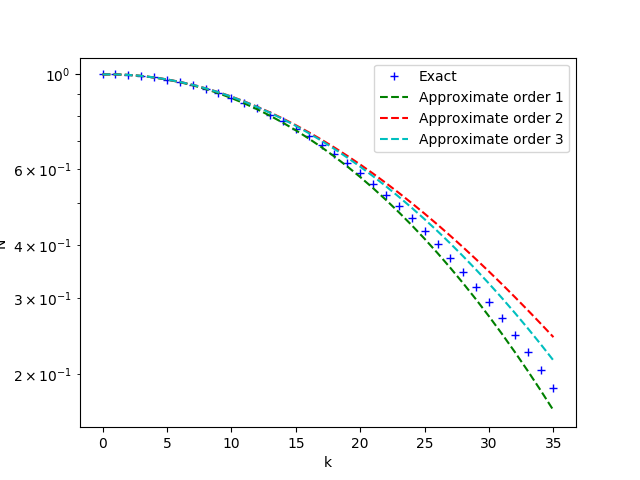
\includegraphics[width=0.7\textwidth]{birthdays/birthdays_approxorder_3.png}
    \caption{Plot of Exact and Approximate Solutions with higher order terms in
        logarithm expansion\label{fig:birthdays_higher_order}}
\end{figure}

Not so great! But this is because we note that our expansion is in order
$\frac{k}{N - k}$, so it's expected that as this approaches unity our expansion
falls apart, which happens when $k = N/2$. A quick exercise replacing the Taylor
expansion with the full exponent recovers the exactly correct curve.

\chapter{05/02/17---L'H\^opital's Rule and Complex Analysis}

This ought to be a short chapter. Had a sudden shower thought to prove
L'H\^opital's rule using complex analysis, let's just carry it out.

Consider if some function $f(x) = \frac{g(x)}{h(x)}$ such that $g(a) = h(a) =
0$. Then the well-known solution to evaluating $f(a)$ is to differentiate both
numerator and denominator until at least one is non-vanishing, then evaluate,
this is \emph{L'H\^opital's Rule}.

Let's try instead to compute the residue of $\frac{f(x)}{x - a}$ at $x = a$.
Now, if $f(x)$ is not singular, then this function has a simple pole at $x = a$
and the residue is simply $f(a)$. Let this be our motivating factor.

Let there be some $h'(x)$ such that $h(x) = (x-a)^nh'(x)$ and $h'(x)$ is
analytic at $a$. Then we know that the residue of $f(x)$ is given
\begin{align}
    \Res(f, a)
        &= \lim_{x \to a}\frac{1}{n!}
            \frac{\mathrm{d}^n}{\mathrm{d}x^n}
            (x - a)^{n+1} f(x)\\
        &= \lim_{x \to a}\frac{1}{n!}
            \frac{\mathrm{d}^n}{\mathrm{d}x^n}
            \frac{g(x)}{h'(x)} \nonumber
\end{align}

There are then two cases when $f(a)$ is analytic:
\begin{itemize}
    \item $g^{(n)} \neq 0$, but all lower-order derivatives vanish. Some trivial
        reapplication of the quotient rule to compute the derivatives shows that
        then
        \begin{align*}
            \frac{\mathrm{d}^n}{\mathrm{d}x^n} \frac{g(x)}{h'(x)}
                &= \frac{g^{(n)}(x)(h'(x))^{2^n - 1}}{(h'(x))^{2^n}}\\
                &= \frac{g^{(n)}(x)}{h'(x)}
        \end{align*}
        but then $h^{(n)}(x = a) = n! h'(x=a)$, and so we find the above result
        agrees with L'H\^opital's Rule.

    \item $g^{(n)} = 0$ and all lower-order derivatives also vanish. Since we
        only differentiate $g(x)$ a maximum of $n$ times, all terms vanish and
        $\Res(f, a) = f(a) = 0$ as also expected.
\end{itemize}

What about when $f(a)$ is singular? Then this means that for some $k < n$,
$f'(x) = f(x)(x - a)^k$ is analytic at $x = a$, and $f'(x)$ must then
also be equal to
\begin{align*}
    f'(x) &= \frac{(x - a)^kg(x)}{(x - a)^nh'(x)}
\end{align*}
and so if we apply L'H\^opital's Rule, we will obtain a diverging result after
only $k$ iterations.

The above proof could be tightened but I'm not going to bother, it seems the
equivalence is pretty clear (at least when $f(x)$ is analytic in a neighborhood
of $a$ and the usual).

How about for $f(x) = \frac{g(x)}{h(x)}$ where $g(x), h(x)$ are both divergent
at $x = a$? This should be a simple exercise if we just take $f(x) =
\frac{1/h(x)}{1/g(x)}$ and perform the above proof on this.

\chapter{05/28/17---Parabolas}

We're hiking the Grand Canyon, and halfway down we rediscover signal that we
did not have at the top. I joke ``clearly it is because the Grand Canyon
approximates a parabolic dish reflector, and since we are now closer to the
focus of the parabola we will have better signal than up top.'' To follow up on
this, we first demonstrate that the parabola has the unique property that all
plane waves of incidence perpendicular to the axis of symmetry of the parabola
reflect off the surface to a particular point, called the \emph{focus}.

We then consider the more interesting problem: if we project the reflections of
incoming rays onto the axis of symmetry, they form a perfect delta function at
the focus if the surface is a perfect parabola. If we want the distribution to
be normally distributed and centered on the focus of the parabola, what
uncertainty tolerances do we have on height measurements of the parabola? More
generally, how do various sources of error (error in parabola parameter, error
in height measurements) propagate to uncertainties in focusing ability?

\section{Parabola Properties}

We wish to find a 1D surface in $\mathbb{R}^2$ that has the following property:
for any ray traveling in the $-\hat{y}$ direction, if the ray reflects according
to the Law of Reflection (symmetric about the normal to the surface at the point
of incidence) then it must go through the \emph{focus}.

Call the \emph{focus} $(0, a)$. Consider also a surface $y(x)$. Then the ray
from the focus to the surface has slope $b(x) = \frac{y - a}{x}$. Thus, we wish
to find $\rd{y}{x}$ such that the normal $-\rd{x}{y}$ \emph{bisects} the angle
formed by $b(x)$ and $\hat{y}$. This implies that the tangent must bisect
$\hat{x}$ and the slope formed by $-\frac{1}{b(x)}$, the normal to $b(x)$.
Calling the angle formed by $\frac{x}{a - y}$ and $\hat{x}$ $2\theta$, then this
implies that
\begin{align*}
    \tan 2\theta &= \frac{x}{a - y} = \frac{2\frac{x}{2a}}{1 - y/a}
\end{align*}

Recall double angle identity $\tan 2\theta = \frac{2\tan \theta}{1 -
\tan^2\theta}$. Making an inspired guess, assume $\left( \frac{x}{2a}
\right)^2 = \frac{y}{a}$, in which case $\tan\theta = \rd{y}{x} = \frac{x}{2a}$,
while additionally $y'(x) = \rd{}{x}\left( \frac{x^2}{4a} \right) =
\frac{x}{2a}$. Wow!

\section{Uncertainties}

It is clear that if the uncertainties are in the parameter $a = a(x)$, then the
distribution of rays along the axis of symmetry will simply be the PDF of $a$
over all $x$, or more quantitatively, calling $L(y)$ the luminosity (density of
rays) incident at $(0, y)$, we have
\begin{align*}
    L(y) &= \int\limits_{-\infty}^{\infty}\delta(y - a(x))\;\mathrm{d}x
\end{align*}
and so if there are random variations in $a$, we can obtain $L(y)$ as well.

What about if the uncertainty is in $y(x)$ though? It seems perhaps sensible to
propagate the uncertainty to $\rd{y}{x}$ and translate that into an uncertainty
on $a(x)$. For example, if $y(x) = y_0(x) + N_{0, \sigma}$ where $N$ is a random
variable with zero mean and $\sigma$ variance, then we know that
\begin{align*}
    \rd{y}{x}
        &= \rd{y_0}{x} + N_{0, \sigma\sqrt{2}}\\
        &= \frac{x}{2a} + N_{0, \sigma\sqrt{2}}\\
        &= \frac{x}{2a} \pm \sigma \sqrt{2}
\end{align*}

We aspire instead to express this uncertainty as one in $a$, so we instead write
$a = a_0 + N_{0, \sigma_a}$. We can rewrite
\begin{align*}
    \frac{x}{2(a_0 + N_{0, \sigma_a})}
        &= \frac{x}{2a_0} \pm \frac{x \sigma_a}{2 a_0^2}
\end{align*}
and matching terms we find $\sigma = \frac{x\sigma_a}{2a_0^2 \sqrt{2}}$.

However, we must consider one more thing: this corresponds to a global
uncertainty on $a$ by $\sigma_a$, and it assumes that the point at some $x$
value has position given by $y(x) = \frac{x^2}{4 (a_0 + \sigma_a)}$ rather than
position $\frac{x^2}{4 a_0}$. This can be remedied: for any given parameter $a =
a_0 \pm N_{0, \sigma_a}$, the position of the focus $(0, y_a)$ is given by
\begin{align*}
    y_a
        &= a + \left(\frac{x^2}{4a_0} - \frac{x^2}{4 a}\right)\\
        &= a_0 + N_{0, \sigma_a} + \frac{x^2}{4a_0^2}N_{0, \sigma_a}
\end{align*}

\chapter{07/16/17---Principal Component Analysis}

My friend and I were watching a Youtube video called ``18 types of Asian girls''
when we both had the same reaction: why 18? As von Neumann famously said, four
parameters fits an elephant, five wiggles its trunk. So instead, we both arrived
at Principal Component Analysis (PCA) as a viable way to determine just how many
categories are needed. And this made me think again about how this technique
works, so I looked up a few definitions.

\begin{description}
    \item[SVD] \emph{Singular Value Decomposition} is a fancy name for
        change of basis, diagonalizing a matrix. In the particular case of a
        rectangular matrix, diagonalizing the matrix means the rectangle becomes
        the concatenation of a diagonal square matrix and a zeroes matrix.

    \item[PCA] \emph{Principal Component Analysis} is looking for linear
        combinations of feature vector components that are strongly correlated
        in a dataset. These linear combinations are the eigenvectors that the
        SVD yields.
\end{description}

In our particular case, consider if we have $N$ Asian girls, each with a
$k$-dimensional feature vector. Then our data $M$ form an $N \times k$ matrix, and
so the SVD $\bm{U\Sigma V}$ consists of three matricies:
\begin{itemize}
    \item $\bm{\Sigma}$ is a $k \times k$ diagonal matrix, with $(N - k) \times
        k$ zero entries concatenated.
    \item $\bm{U}$ is $N \times N$, but obviously in each row only the first $k$
        values matter, since the remainder are being multiplied by the zero
        entries of $\Sigma$
    \item $\bm{V}$ is a $k \times k$ matrix, the $k$ eigenvectors that go into
        the PCA\@. Generally we expect only a few of these to correspond to larger
        eigenvalues, and these are the principal components we expect.
\end{itemize}

As a demonstration, let's try!

Conclusion from my demonstration: Forgot that PCA and clustering are different.
Oops. Probably not gonna resume this one.

\chapter{08/15/17---Sum until $> 1$}

Sum random numbers uniformly distributed $\in [0,1]$ until you exceed $1$.
What's the expected value of the number you end up with?

\section{Simulation}

We can first simulate, as in \autoref{fig:sumToOne10e6}. The simulation
concludes that the mean is pretty close to $\frac{e}{2}$. The Python code used
is:
\lstinputlisting[basicstyle=\ttfamily\scriptsize, language=python]
{sumToOne/sim.py}
\begin{figure}[H]
    \centering
    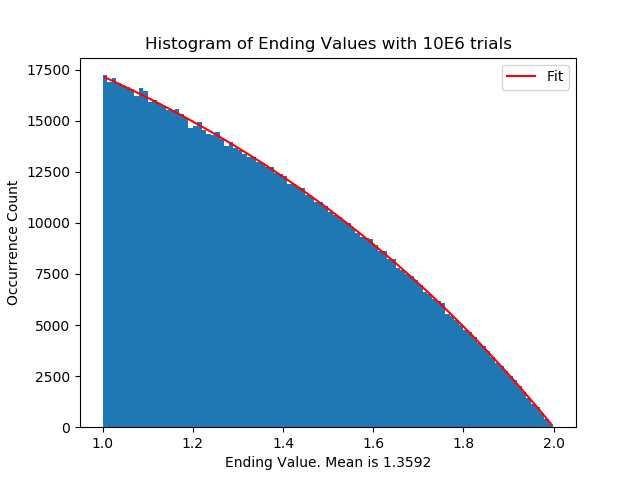
\includegraphics[width=0.8\textwidth]{sumToOne/trials10e6.png}
    \caption{Simulation with $10^6$ data points.\label{fig:sumToOne10e6}}
\end{figure}

\section{Solution}

So what's the theory behind this?

The probability that you to take $> k$ additions to exceed $1$ is the
probability that $k$ $U_0^1$ numbers sum to $\leq 1$. This is the volume of the
volume formed by the origin and each of the unit vectors in $k$ dimensions, also
$\frac{1}{k!}$ (lemma coming).

Given this, the probability that we exceed exactly on the $k$th addition is the
probability that we have not yet succeeded by the $k-1$th addition ($1/(k-1)!$)
but subsequently fail by the $k$th addition. The probability that we \emph{do
not} fail on the $k$th addition is $1/k!$, but everything that does not fail on
the $k$th addition also does not on the $k-1$th addition, so the probability
that we do not fail on the $k$th addition conditional on not failing on the
$k-1$th addition is just $1/k$, from which we easily deduce that \emph{failing}
on the $k$th addition is $(k-1)/k!$.

Then, the expected number of additions is just $\sum\limits_{k}^{} k P(k)$ where
$P(k)$ is the probability of terminating exactly on the $k$th addition as
computed above. The sum starts at $k=2$ since this is the first point at which
we can first exceed $1$, and so we have $\E =
\sum\limits_{k=2}^{\infty}\frac{1}{(k - 2)!} = e$. Then, since each addition
contributes on average $1/2$, we have that the expected value is $e/2$.

\subsection{Lemma}

\textbf{Claim:} In $D$ dimensions, the volume of points satisfying $q_k \geq 0$
and $\sum\limits_{k=1}^{D} q_k \leq a$ has volume $\frac{a^D}{D!}$.
Geometrically, it is the volume bound by the origin and the points distance $a$
along each of the $D$ dimensions (i.e.\ $(a,0,0,\dots), (0,a,0,\dots)$).

\textbf{Proof:} We prove via induction. The base case is simply $D=1$, in which
case the line segment of length $a$ has length $a = \frac{a^1}{1!}$.

Inductively, let $V_D(a)$ be the volume in $D$ dimensions summing to $\leq a$.
Then we notice that $V_D(a)$ is just the sum of all $V_{D - 1}(a')$ where $0
\leq a' \leq a$ multiplied by some thickness $\mathrm{d}a'$. But since $\int
\frac{a^{D - 1}}{D!} \mathrm{d}a = \frac{a^D}{D!}$ we are done.

This proves the result we used where the volume is $\frac{1}{D!}$.

To be fair, this is a fairly trivial result if we use the result that
$\norm{\bigwedge_k a\hat{e}_k}$ is the above described volume, since the norm of
the wedge product is the $1/D!$ times the determinant of the matrix containing
the basis vectors, and the matrix is just $a \mathbb{I}_D$ where $\mathbb{I}_D$
is the identity matrix in $D$ dimensions.

\subsection{Distribution}

A much more interesting problem is deriving the distribution that we found in
the simulation!

Consider $P_k(x)$ the probability of being on value $x$ after exactly $k$
additions. The probability of ending on some value $x_f$ is then
\begin{align}
    P_k(1 \leq x_f \leq 2) &= \int\limits_{x_f - 1}^{1}P_{k - 1}(x_i)\;\mathrm{d}x_i
\end{align}

But we know from above that $P_{k - 1}(x_i) = \frac{(x_i)^{k - 2}}{(k - 2)!}$
since this is the PDF, we must differentiate one time from the CDF\@. Then,
summing over all $k$, we have that
\begin{align}
    P(1 \leq x_f \leq 2) &= \int\limits_{x_f - 1}^{1}P(x_i)\;\mathrm{d}x_i\\
        &\propto \int\limits_{x_f - 1}^{1}e^{x_i}\;\mathrm{d}x_i\\
        &\propto e - e^{x_f - 1}
\end{align}

Normalization is a bit tricky to get from first principles since there's some
``leakage'' when summing over $P(x_i)$, but we can always just normalize
$P(x_f)$ directly instead. The fit is shown in \autoref{fig:sumToOne10e6}.

\chapter{8/18/2017---Random Processes}

Motivated by stock prices. Consider if for every price $P_1$ there is a
time-independent probability $\Delta(P_2, P_1)$ of transitioning to $P_2$
from $P_1$. Compute the PSD of the random trajectories this produces.

The analysis is most easily carried out by looking at mixed states of prices.
Consider a state $\ket{\psi} = \sum\limits_{k=1}^{N} a_kP_k$ that is an
eigenvector of $\Delta$, such that $\Delta\ket{\psi} = \ket{\psi}$
(let's assume $N$ the number of states is finite for now). The significance of
such a state is that if we choose $M \gg N$ prices, distributed with
$\dotp{P_k}{\psi}$ probability distribution, then the distribution after the
action of $\Delta$ is still $\ket{\psi}$.

The way that we capture the ``transition with probability'' is as follows:
suppose you start at some value $P_0$, then apply $\Delta$ a few, $q$,
times. Then the probability of measuring each of the $P_k$ prices is simply
$P[P_k] = \bra{P_k}\Delta^q\ket{P_0}$, just like in quantum mechanics.

Thus, decompose any initial state $\ket{\varphi_0}$ (which may be a pure state)
into some sum of eigenvectors $a_j\ket{\psi_j}$. Then at some future time $t$
the probability of finding $\ket{\varphi_t}$ in state $P_k$ is given simply
\begin{align}
    P[\varphi_t = P_k]
        &= \sum\limits_{j}^{} \bra{P_k}\Delta^t a_j\ket{\psi_j} \nonumber\\
        &= \sum\limits_{j}^{} a_j\dotp{P_k}{\psi_j}
\end{align}

This is not very helpful to us though, since to compute any spatial correlations
we have to discount spurious transitions (e.g.\ in a random walk, one cannot go
from $t=1, x=-1$ to $t=2, x=2$, but by simply integrating the probability
distribution such contributions are included). We'll have to find something more
clever.

To compute the PSD, we look to the autocorrelation. Recall that the PSD of a
continuous signal $f(t)$ is given by the FT of the autocorrelation, defined to
be
\begin{align}
    R_{ff}(\tau) &\propto \int\limits_{-\infty}^{\infty}f(u + \tau) f(u)
        \;\mathrm{d}u.
\end{align}

\chapter{10/16/17---Hopping Bunny}

A bunny in two dimensions takes three hops of unit distance in random
directions. What's the probability the bunny ends up within unit distance of its
starting position?

\section{Simple Solution}\label{s:10/16/17.simple}

Label the points that the bunny hops to be labeled by $P_i$ and the circles of
unit radius about each of the $P_i$ be labeled $C_i$. Let $P_0$ be the origin,
then $P_1$ must lie on the unit circle $C_0$. WLOG choose $P_1 = (0, 1)$.

Now, we know that $P_3$ must lie on $C_2$, and the
probability that $P_3$ lies inside the unit circle is the arclength of $C_2$
inside $C_0$. We can draw diagram \autoref{fig:10/16/17.circles}.
\begin{figure}[!h]
    \centering
    \begin{tikzpicture}[scale=2]
        \filldraw[black] (0, 0) circle(0.05);
        \node[below] at (0, 0) {$P_0$};
        \filldraw[black] (0, 1) circle(0.05);
        \node[below] at (0, 1) {$P_1$};
        \filldraw[black] (0.85, 1.5) circle(0.05);
        \node[below] at (0.85, 1.5) {$P_2$};
        \draw (0, 0) circle(1);
        \draw[dashed] (0.85, 1.5) circle(1);
    \end{tikzpicture}
    \caption{Schematic drawing of the argument for \autoref{s:10/16/17.simple}.}
\end{figure}\label{fig:10/16/17.circles}

We note that if we define $\theta$ to be the angle formed by $P_0$--$P_1$--$P_2$
then the intersection of $C_2, C_0$ has arclength $\abs{\pi - \theta}$. Thus,
the probability given $\theta$ of ending up inside $C_0$ is $\frac{\abs{\pi -
\theta}}{2\pi}$. Then since $\theta$ ranges uniformly over $[0, 2\pi]$, we
simply average and find probability $P$ of ending up inside $C_0$ to be
\begin{equation}
    P = \frac{1}{2\pi}\int\limits_{0}^{2\pi}\frac{\abs{\pi - \theta}}{2\pi}
        \;\mathrm{d}\theta
        = \frac{1}{4}.
\end{equation}

\section{Generalizable Solution}

Let's develop a more powerful solution capable of explaining the probability
trends in two dimensions:
\lstinputlisting[basicstyle=\ttfamily\tiny]{bunny/2sim.dat}
and three dimensions:
\lstinputlisting[basicstyle=\ttfamily\tiny]{bunny/3sim.dat}

\subsection{Computing $P_n(r)$}

We wish to compute a general formula for $P_n(r)$, the probability distribution
of $r$ after $n$ jumps. To compute this, WLOG suppose we are at a point $(a, 0)$
and we wish to compute the probability that we jump to a distance $r$ away. We
note that $r, a$ are related by
\begin{align}
    r^2 &= a^2 + 1 - 2a\cos\theta,\\
    \mathrm{d}r &= \frac{r}{2a\sin\theta}\mathrm{d}\theta,\\
    P(r|a) &= P(\theta)\rd{r}{\theta},\nonumber\\
        &= \frac{1}{2\pi} \frac{r}{2a\sin\theta},\nonumber\\
        & = 2\frac{1}{2\pi}\frac{r}{2a\sqrt{1 - \left(
            \frac{r^2 - a^2 - 1}{2a}
        \right)^2}},\label{eq:10/16/17.sol}
\end{align}
where a factor of $2$ arises since there are two values of $\theta$ that can
satisfy the given square root.

But this means that we can just integrate over all $a$ given an existing
$P_{n-1}(a)$ to obtain $P_n(r)$, namely
\begin{equation}
    P_n(r) = \int\limits_{0}^{n - 1}
        P_{n - 1}(a) 2\frac{1}{2\pi}\frac{r}{2a\sqrt{1 - \left(
            \frac{r^2 - a^2 - 1}{2a}
        \right)^2}}\;\mathrm{d}a.
        \label{eq:10/16/17.recursive}
\end{equation}

We can verify this expression by computing explicitly $P_2(a)$, since $P_1(a) =
\delta(1)$. We first compute it from scratch then take the limit of
\autoref{eq:10/16/17.sol} to verify that the two expressions agree. First
\begin{align}
    r^2 &= 2 - 2\cos \theta & r = 2\sin\frac{\theta}{2},\\
    \mathrm{d}r &= \cos \frac{\theta}{2}\mathrm{d}\theta,\\
    P_2(r) &= \frac{1}{2\pi} \frac{1}{\cos \frac{\theta}{2}},\nonumber\\
        &= 2\frac{1}{2\pi}\sqrt{\frac{1}{1 - \left( \frac{r}{2} \right)^2}}.
\end{align}

It is clear that $\int\limits_{0}^{1}P_2(r)\;\mathrm{d}r$ must be $\frac{1}{3}$,
since $C_1$ must have arclength $\frac{\pi}{3}$ inside $C_0$, and indeed
performing the integral we obtain this result.

We then need to set $a = 1$ in \autoref{eq:10/16/17.sol}. This gives us
\begin{align}
    P(r|a = 1) &= 2\frac{1}{2\pi}\frac{r}{2\sqrt{1 - \left(
        \frac{r^2 - 2}{2}
    \right)^2}},\nonumber\\
        &= \frac{r}{2\pi} \frac{1}{\sin\theta} = \frac{1}{2\pi}\frac{1}{\cos
        \frac{\theta}{2}}.
\end{align}
The results thankfully agree!

\subsection{Computing $P_n$}

Define $P_n = P_n(r < 1)$. Now, we do some seriously hacky algebra. We can
express $P_n$ in terms of \autoref{eq:10/16/17.recursive} as follows
\begin{equation}
    P_n = \int\limits_{0}^{1}\int\limits_{0}^{2}P_{n - 1}(a)
        2\frac{1}{2\pi} \frac{r}{\sqrt{1 - \left( \frac{r^2 - a^2 - 1}{2a}
        \right)^2}}\;\mathrm{d}a\mathrm{d}r.
\end{equation}
We know that we only need to integrate out to $a = 2$ since any larger cannot
produce $r < 1$.

We exchange the order of integration and perform the $r$ integral first. We
recognize the integrand to be of form $-\frac{f'(x)}{\sqrt{1 - f(x)}}$ which
integrates to a $\sin^{-1}$, or more precisely
\begin{equation}
    P_n = -\int\limits_{0}^{2}P_{n - 1}(a)
        \frac{1}{2\pi} \arcsin \left[
            \frac{r^2 - a^2 - 1}{2a}
        \right]_0^1\;\mathrm{d}a.
\end{equation}

Now we drop the $r = 0$ evaluation since it's just evaluating the CDF at the
lower boundary (I agree it's scary that the integrand doesn't seem to vanish
stop giving me a hard time), then the integrand simplifies to
\begin{equation}
    P_n = \int\limits_{0}^{2}P_{n - 1}(a)
        \frac{1}{2\pi} \arcsin \frac{a}{2}\;\mathrm{d}a,
\end{equation}
Now, just to verify this expression, let's evaluate for $n = 3$ using our
$P_2(a)$ that we have from before. This integral is then
\begin{align}
    P_3 &= \int\limits_{0}^{2}\frac{1}{2\pi^2}
        \sqrt{\frac{1}{1 - \left( \frac{a}{2} \right)^2}}
        \arcsin \frac{a}{2}\;\mathrm{d}a,\nonumber\\
        &= \int\limits_{0}^{1}\frac{1}{\pi^2}
            \sqrt{\frac{1}{1 - \left( \frac{a}{2} \right)^2}}
            \arcsin \frac{a}{2}\;\mathrm{d}\frac{a}{2},\nonumber\\
        &= \frac{1}{\pi^2} \arcsin^2 x\Bigg|_{x=0}^{x=1},\nonumber\\
        &= \frac{1}{4}.
\end{align}

So technically this is prescriptive. And we can feasibly see that the successive
antiderivatives might go something like $\arcsin^{n-1}(x)$ which somehow
fortuitously yields a $\frac{1}{n + 1}$ relationship? At least there is
something linearly increasing. But this is far beyond our algebraic abilities
sadly.

\chapter{10/22/17---Other Leaping Bunny}

A bunny starts at $x = 0$ on the one-dimensional real number line. Each time
step, it jumps with constant integer $v$ (positive or negative) to a new integer
position. You can only examine one $x$ value at each time. Find the bunny in
finite time.

\section{Rigorously Defining ``In Finite Time''}

What does it mean to find the bunny in finite time? This means that given an
initial bunny velocity $v < V$, we are guaranteed to find the bunny in some time
$t < T(V)$ where $T(V)$ is finite for all finite $V$.

\section{Positive Velocity Starting at Origin}

Consider if we are given integer $v \geq 0$. Then for any given $t$, we examine
what position the bunny would be at if $v = t$. This means at time $t = 0$, we
examine $x = 0$ because $x = vt = 0 \times 0 = 0$. At $t = 1$, we examine $x =
4$ because $x = vt = 1 \times 1 = 1$, and so on.

\section{Integer Velocity Starting at Origin}

This is a bit trickier; we obviously cannot examine all positive $v$ then all
negative $v$ since then if $v$ is negative we will not find it in finite time!
Instead, we search as follows: for odd $t = 2\tau - 1$, we search as if $v =
-\tau$, and for even $t = 2\tau'$ we search as if $v = \tau'$.

We prove that the bunny velocity can be found in finite time: for a bunny
velocity $v < V$, we are guaranteed to find the bunny in $t < 2\abs{V}$ time,
and since $T(V) = 2\abs{V}$ we guarantee that for any finite bunny velocity we
find the bunny in finite time. After the bunny is found, the position of the
bunny one-to-one maps to the $v$ of the bunny, so the bunny velocity can be
computed in constant time as well.

This follows the same train of thought as Cantor cardinality counting arguments:
two sets are of the same cardinality if for any finite member of one we can
determine to which member of another it corresponds in finite time, very
intuitively and roughly.

\section{Integer Velocity, Unknown Integer Initial Position}

The initial conditions for the bunny live in some countable configuration space
$(x_0, v)$, i.e.\ given $x_0, v$ of the bunny we can determine for any time
where the bunny is located. We need to map a linear search $t$ to this
configuration space. The intuitive algorithm suffices; within time $t \in [k^2,
k + 1^2]$ time for some $k$, we search over rectangular perimeter $(k/2,
-k/2)$--$(k/2, k/2)$--$(-k/2, k/2)$--$(-k/2, -k/2)$--$(k/2, -k/2)$. This traces
out a spiral in $(x_0, v)$ space. Then of course at each $(x_0, v)$, we examine
the position the bunny would be found at.

However, this problem is harder than the previous problem; once we have located
the bunny, we cannot invert to find the initial $(x_0, v)$ because the map
$(x_0, v) \to x$ is not injective and hence not invertible! More precisely, the
map is many-to-one, since multiple $(x_0, v)$s can end up at a given position
$x$ where we find the bunny, even for a constant time.

However, once we have found the bunny once, we can let this position $x$ be the
new origin, then this problem reduces to the previously solved problem, bunny
starting at the origin with integer velocity, and we can apply our previous
algorithm to compute $v$ and disambiguate between the degenerate $(x_0, v)$
incurred by the previous step.

We prove that this finds the bunny in finite time: for any bunny in
configuration space bound by $\abs{x_0} < X, \abs{v} < V$, we are guaranteed to
find the bunny in time $t < 4\max(X, V)^2$ which is finite for all finite values
of $X, V$ (this is the natural extension of the earlier ``finite time''
definition now that configuration space is larger), thus for any finite initial
position and velocity the bunny can be found in finite time. Then, once the
bunny is found, the second step to determine $v$ has also been proven to take
finite time for finite $v$, therefore we are guaranteed to determine the bunny's
velocity $v$ in finite time.

This can obviously be generalized to any countable configuration space, giving
some more intuition to Cantor's notion of \emph{countable sets} having
equivalent cardinality.

\chapter{02/04/18---Conformal Mapping}

Conformal maps locally preserve angles.

\section{Reviewing Analytic Functions as Conformal Maps}

Consider an analytic function $f: \mathbb{C} \to \mathbb{C}$, and write $w =
f(z)$. We wish to see what happens to angles in the $z$ plane under the action
of $f$. Angles are a local property, so we expand $f(z)$ about some local point
$z_0$ in a Taylor series
\begin{align}
    f(z_0 + \Delta z) &\approx f(z_0) + \sum\limits_{k=1}^\infty
        \frac{f^{(k)}(z_0)}{k!}\p*{\Delta z}^k,\\
    \Delta w &= \sum\limits \frac{f^{(k)}(z_0)}{k!}\p*{\Delta z}^k,
\end{align}
where $\Delta w = f(z_0 + \Delta z) - f(z_0)$. For small $\Delta z$, it's clear
that $\Delta w$ is set by the leading order in the summation above.

Notably, if $f'(z_0) \neq 0$ then we have $\Delta w = f'(z_0) \Delta z$. In this
case, $\abs{\Delta w} = \abs{f'(z_0)}\abs{\Delta z}$ while $\Arg \Delta w = \Arg
f'(z_0) + \Arg \Delta z$. It is of worth to note that it preserves relative
lengths (two $\Delta z$ of the same length produce two $\Delta w$ of the same
length) though not area, and that it preserves angles (two $\Delta z$ with
different arguments will correspond to two $\Delta w$ that differ by the same
argument).

If $f'(z_0) = 0$, then the relation between $\Delta w$ and $\Delta z$ is more
complex; namely $\Delta w = \frac{f^{(k)}(z_0)}{k!} (\Delta z)^k$ for a $k$-th order
zero $f(z_0)$. We still have shape-preserving properties, but angles are
\emph{enlarged} in $w$ space, $\Arg \Delta w = \Arg f^{(k)}(z_0) + k \Arg \Delta
z$.

\section{Complex Analysis and Conformal Mapping}

It was mentioned in the book I'm reading out of, Churchill \emph{Complex
Variables and Applications}, that conformal mapping is only used in 2D problems.
One naturally wonders why conformal mapping is restricted to 2D\@; one can
easily imagine e.g.\ why should quaternions not be able to extend conformal
mapping to 4D domains?

This turns out to be \emph{Liouville's Theorem}, for which the proof is
sufficiently complicated it is not outlined on Wikipedia \frownie. But I think
we can get some understanding of the factors at play.

Consider two vector spaces $V, W$ and a function $f: V \to W$. By choosing
vector spaces for our domain and range, we guarantee that members of $V, W$ are
closed under addition and scalar multiplication. Furthermore, in the context of
conformal mapping, endow both $V, W$ with an inner product satisfying linearity,
which we will denote by $\expvalue{u, v}, u, v \in V$ such that $\expvalue{u, u}
\neq 0$ unless $u = 0$.

With this structure, we are able to introduce \emph{components}. Call two
vectors $\expvalue{u, v} = 0$ \emph{orthogonal}. For vector space $V$, consider
the maximal set of vectors that are pairwise orthogonal and have norm $1$; call
these $\expvalue{e_i e_j} = \delta_{ij}$ (we will take the set to be finite for
now, but natural extensions follow for countably infinite and continuously
infinite sets I imagine). Then, by linearity, vectors $v \in V$ can be written
$\sum\limits_i v_ie_i$; this is obviously possible by decomposing $v$ into two
other vectors $v_1, v_2$ such that $\expvalue{v_1 e_i} = 0, \expvalue{v_2e_j} =
0 \forall j \neq i$, doable since the $\z*{e_i}$ are maximal. It is then obvious
that $\expvalue{u, v} = \sum\limits_i u_iv_i$, and we have our usual dot
product.

What this shows is that \emph{the linear norm for a vector space is necessarily
an $\mathcal{L}^2$ norm}. In fact, any bilinear form on the vector space is
necessarily quadratic in the components of an arbitrarily vector in a spanning
basis of the bilinear form. If we only definitions of angles that only use two
vectors from $V$ in a bilinear form (e.g.\ $\cos\theta = \expvalue{u, v}$), then
any angle-preserving transformation must preserve the $\mathcal{L}^2$ norm of
elements of $V$. This is in agreement with Liouville's Theorem which basically
restricts conformal mappings in Euclidean space to mappings that are conformal
in $2D$. Of course, my result assumes one only uses angles related to a bilinear
form, but that seems reasonable from a practical perspective.

It lastly bears noting that our requirement that $V, W$ have an inner product
satisfying linearity is natural. Only a vector space with a linear inner product
exhibits notions of proximity, and we want to study ``close'' to some vector
$v_0$ to employ linearization such as the Taylor Series.

Thus, we see that angle-preserving transformations can only operate in a 2D
slice of a higher dimensionality system and no generalizations to higher
dimension systems can capture additional complexity. This is obviously not meant
to be a proof, but it seems reasonably clear that performing an analysis like
the one we do above can only be done in 2D topologies.

\section{Harmonic Functions and Conformal Mappings}

Recall a harmonic function $u(x, y)$ satisfies Laplace equation $\nabla^2 u =
0$. We can show that there exists another harmonic function $v(x, y)$ such that
$u + iv$ is analytic in $z = x + iy$; this is just inverting the Cauchy-Reimann
conditions. Thus, a function being harmonic over a domain is equivalent to the
sum of it and its harmonic conjugate being analytic over the same domain.

Harmonic functions are important because they crop up everywhere, with Neumann
or Dirichlet BCs. It's also important that every harmonic function of $z = x +
iy$ is also harmonic under change of variables $z = f(u + iv)$ if $f$ is
analytic; the proof follows because for the harmonic function, there is a
harmonic conjugate that makes it an analytic function of $z$ and ergo of $u +
iv$, which forces the original harmonic function te be harmonic in $u + iv$ as
well.

Finally, to finish applying conformal mappings to harmonic functions, we must
study how boundary conditions map. It turns out that Dirichlet and Neumann BCs
for a function $H(x, y)$ on a \emph{level curve} (curve where $H(x_c, y_c) = C$)
are unchanged under conformal mapping; $H$ will be constant on the image of the
level curve.

Consider a boundary parameterized by $p(s)$, whose image boundary is $f(p(s))$.
Then at some $p(s_0)$ and neighboring point $p(s_0 + \Delta s)$, the harmonic
function $H$ takes on value $H(s_0), H(s_0 + \Delta s)$, their difference
being approximately $H'(s) \Delta s$. Under conformal mapping $w = f(z)$,
path $p(s)$ maps to $p'(\sigma)$ where $\sigma$ the new path length is related
to the old by $\sigma = \abs{\rd{w}{z}}s$. Thus the new path length difference
is $\rd{H}{\sigma} = \rd{H}{s}\abs{\rd{w}{z}} \neq \rd{H}{s}$ unless $\rd{H}{s}
= 0$, exactly a level curve.

\section{Conformal Mapping and Laplace's Equation, Examples}

Let's consider trying to compute steady-state $T(x, y)$, when $T(x = \pm \pi/2)
= 0$, $T(y = 0) = 1$ and $T(x, y) < \infty$ everywhere (equivalently, $T(y \to
\infty) \to 0$), in the semi-infinite slab. With no heat sources, $T$ must
satisfy $\nabla^2 T = 0$ in the steady state limit. Of course, we could solve
using separation of varibables and obtain a series solution, but there is a
slicker solution.

Let $z = x + iy$. We consider a two-step transformation: $z' = \sin z$ maps the
semi-infinite slab in $z$ to the half plane $y' > 0$ onto . Then $w = \Log
\frac{z' - 1}{z' + 1}$ maps the half plane $y' > 0$ onto an infinite horizontal
slab $w = u + iv, v \in [0, \pi]$.

Let's now keep careful track of where the boundaries of the original $z$ domain
map to. In $z'$, it is clear that the real axis of the $z$ domain maps to the
$x' \in [-1, 1]$ region in $z'$ as well. The other two boundaries, $z = \pm 1 +
iy, y > 0$ map to $z' = x, \abs{x} > 1$. Thus, $T(z') = 1$ on the real axis
between $[-1, 1]$ and is zero along the rest of the real axis.

Then, when making the $w$ mapping, the two boundaries $w = u, w = u + i\pi$, we
note that $\Re(z') \in [-1, 1]$ maps to $w = u + i\pi$ and the remainder of the
axis maps to $w = u$. Thus, $T(u) = 0, T(u + i\pi) = 1$.

Now, a simple harmonic function that is bounded in the strip and satisfies the
boundary conditions is just $T(w) = \frac{v}{\pi} = \frac{\Im(w)}{\pi}$. We note
that it is level on the boundary (to satisfy the BCs) and is bounded in the
domain. Inverting the transformations gives us
\begin{align}
    T(w) &= \frac{\Im(w)}{\pi},\\
    T(z') &= \frac{1}{\pi}\arctan \frac{2y'}{x'^2 + y'^2 - 1},\\
    T(z) &= \frac{2}{\pi} \arctan \frac{\cos x}{\sinh y}.
\end{align}

It is worth noting that if we do not require $T$ remain finite at infinity, we
could have added any homogeneous solution to $T(w)$; one class of such functions
are $T(u, v) = \sin nv e^{\pm nu}$, obtained by a simple separation of variables
ansatz. Inverting this to find its effect on $T(z)$ is a bit too much work for
the aging author, but the book's example of $T(z) [ + A\sin z]$ suggests this
will map to some class of functions $A \sin nz$ or the ilk.

\chapter{10/05/18---Plane Boarding}

Anybody that has boarded a plane knows that one always has to wait for the
person in front to put up their bag before getting a seat. It's so infuriating!
So, on a flight right now, let's give some thought to how we might treat this
mathematically.

\section{Counting Inversions}

Let's think about the simplest problem: given a sequence $x_i$ of $N$ numbers,
consider an \emph{inversion} to be a subsequence $x_i < x_{i + 1}$, a
discrepancy from being sorted in descending order. This is of course motivated
by the fact that, if everybody in the back of the plane boarded first, there
would be no waiting for people in front of you (assuming each row has only one
seat). What is the distribution of inversions?

Well, it should be obvious first that you expect $\frac{N - 1}{2}$ inversions:
each subsequence of length $2$ is either ordered or not ordered, with
probability $1/2$, and so by linearity of expectation we expect $\frac{N -
1}{2}$ inversions. By another argument, if we flipped the definition of
inversion, there is exactly one other sequence (reversing the numbers) that
contributes to the original inversion definition in the exact same way. Thus,
the definition of an inversion should not depend on the sign, and so the average
number of inversions must be exactly half so that they sum to be $N - 1$ the
total number of subsequences.

Additionally, since each $X_i$ seems to be  just a Bernoulli process, the
variance is $p(1 - p) = \frac{1}{4}$, and so the standard deviation of the
distribution should be $\frac{\sqrt{N - 1}}{2}$. Instead, the standard deviation
seems to be $\sqrt{(N - 1) / 12}$! See \autoref{fig:inversions}.
\begin{figure}[t]
    \centering
    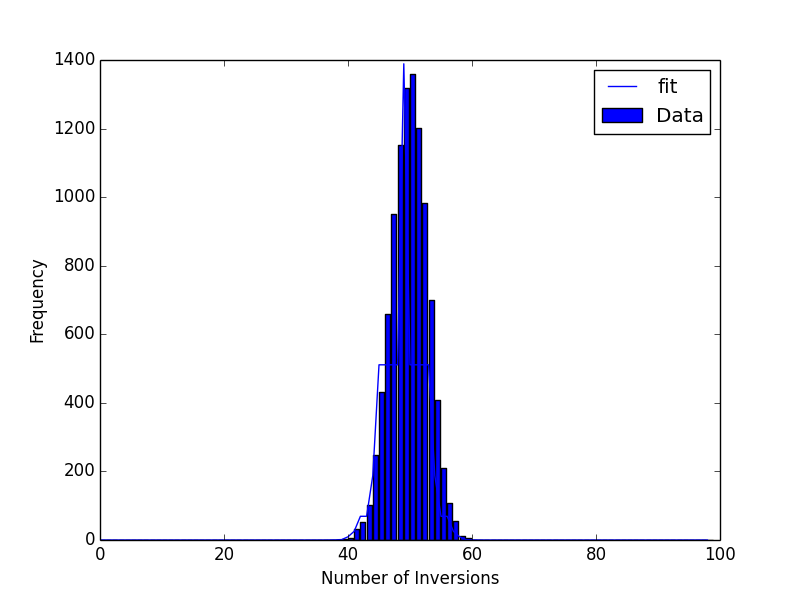
\includegraphics[width=0.6\textwidth]{plane_boarding/inversions.png}
    \caption{Histogram of inversions, fitted with $\mu = \frac{N - 1}{2},
    \sigma^2 = \frac{N - 1}{12}$.}\label{fig:inversions}
\end{figure}

I'm not sure what the discrepancy is for the time being.

\section{Number of people to sit}

This is a slightly more involved problem and a bit more realistic: if everybody
in front of you in line has a seat number further to the back, you can sit!
Thus, if we have a sequence $x_i$ of $N$ numbers, a number $x_i$ can sit
\emph{if it is smaller than every number before it}.

The problem may seem more intimidating, but a closed formula exists. Consider
the first person on line, this person always can sit. Of the remaining people,
everybody who is larger than the first person is immediately ineligible; only
those who are smaller can continue to be eligible for a seat. The first person
is equally distributed among the $N$ possible values, and so letting $f(n)$ be
the expected number of people that can sit of a total of $n$, we may write down
recursive formula
\begin{equation}
    f(n) = \frac{1}{n}\sum\limits_{m = 1}^n f(n - m) + 1.\label{eq:plane.anal}
\end{equation}
The base case of the recursive formula is just $f(0) = 0$, with no people in
line, nobody can be seated. We may examine the agreement of this recursive
formula in \autoref{fig:plane.anal}.
\begin{figure}[t]
    \centering
    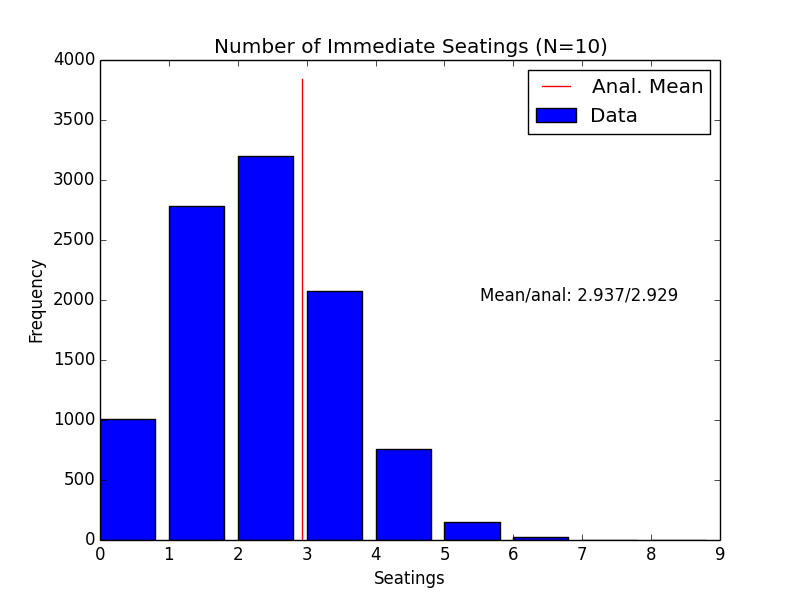
\includegraphics[width=0.6\textwidth]{plane_boarding//seatings.png}
    \caption{Agreement of \autoref{eq:plane.anal} with simulation.
    }\label{fig:plane.anal}
\end{figure}

Of course, of interest is evaluation of \autoref{eq:plane.anal} in closed form.
Perhaps easiest is to observe that $(n - 1)f(n - 1) - (n - 1) = \sum\limits_{m =
1}^{n - 1}f(n - m)$, and so $f(n) - 1 = \frac{1}{n}\s*{f(n - 1) - \frac{n -
1}{n}}$, or $f(n) = f(n - 1) + \frac{1}{n}$! This is easily $f(n) =
\sum\limits_{m = 1}^n \frac{1}{m}$. This agreement can be seen in
\begin{figure}[t]
    \centering
    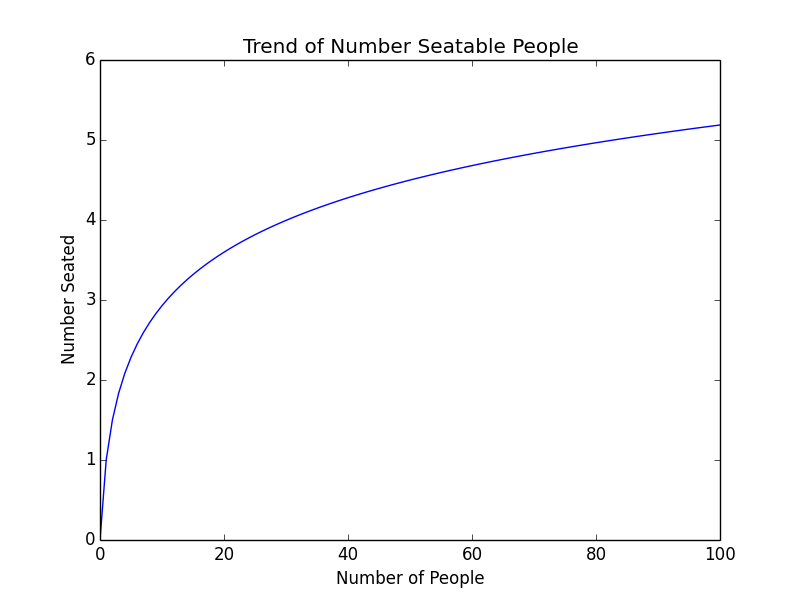
\includegraphics[width=0.6\textwidth]{plane_boarding/seating_trend.png}
    \caption{$f(n)$ evaluated using the recursive formula. The harmonic sum is
    evident in the logarithmic increase.}\label{fig:plane.trend}
\end{figure}

In hindsight, this is another instance of the power of linearity of expectation:
suppose you add people to the line randomly in decreasing order, then for each
subsequent person, there is a $1/m$ probability they're placed at the front of
the line, if they're the $m$th addition.

This has a simple relation to wait times: unlike a geometric series, e.g.\ where
$n/k$ of the people at each iteration get to be seated for some number $k$, we
can only seat $\ln n / n$. This will be a reasonably large number for small
lines, but as the line grows the number of people we can seat \emph{decreases}
rather than increasing as in exponential decay. So longer lines are actually
increasingly inefficient in this model.

\chapter{06/29/19---Research Learning}

\section{Collisionless Boltzmann Equation in Galaxies: Landau Damping}

Inspired by \url{https://arxiv.org/pdf/1906.08655.pdf}. The problem is basically
formulated as thus: consider a kinetic-theoretic description of a fluid using
distribution function $f(t, x, p)$ which obeys collisionless Boltzmann equation
$\rd{f}{t} = 0$ (we use $p$ instead of $v$ to work in Hamiltonian coordinates).
Introducing a periodic perturbation to this fluid results in a singular
dispersion relation, which can be resolved via the usual Landau prescription
(consider a perturbation having grown from zero at $t=-\infty$). The dispersion
relation describes \emph{Landau damping} (or growth), in which energy from the
fluid is exchanged with the perturber.

\subsection{Linearized EOM}

The point of the paper is instead to analytically compute the impact of the
perturber on the distribution function, to quantify the \emph{scarring} of a
galaxy upon encounters with a nearby perturber. The equations of motion coupling
the distribution function and gravitational potential are given
\begin{equation}
    \rd{f}{t} = \pd{f}{t} + \z*{f, \mathcal{H}} = 0,
\end{equation}
where $\mathcal{H} = \frac{p^2}{2} + \Phi$ and $\z*{\dots}$ denotes the Poisson
bracket $\z*{f, \mathcal{H}} = \vec{\nabla}_xf \cdot \vec{\nabla}_p \mathcal{H}
- \vec{\nabla}_pf \cdot \vec{\nabla}_x\mathcal{H}$.

If we linearize for perturbation quantities $f_1, \Phi_1$ where $\Phi_1(x)$ does
not depend on the momenta, we obtain
\begin{align*}
    0 &= \pd{f_1}{t} + \z*{f_1, \mathcal{H}_0}
            - \vec{\nabla}_pf \cdot \vec{\nabla}_x \mathcal{H}_0,\\
        &= \pd{f_1}{t} + \vec{\nabla}_x f_1 \cdot \vec{p}
            - \vec{\nabla}_p f_1 \cdot \vec{\nabla}_x \Phi_0
            - \vec{\nabla}_p f_0 \cdot \vec{\nabla}_x \Phi_1.
\end{align*}

\end{document}
